% \documentclass[aspectratio=169,notes]{beamer}
\documentclass[aspectratio=169]{beamer}
\usetheme[faculty=phil]{fibeamer}
\usepackage{polyglossia}
\setmainlanguage{english} %% main locale instead of `english`, you
%% can typeset the presentation in either Czech or Slovak,
%% respectively.
\setotherlanguages{russian} %% The additional keys allow
%%
%%   \begin{otherlanguage}{czech}   ... \end{otherlanguage}
%%   \begin{otherlanguage}{slovak}  ... \end{otherlanguage}
%%
%% These macros specify information about the presentation
\title[AGLA1]{Analytical Geometry and Linear Algebra I, Visiting Lecture} %% that will be typeset on the
\subtitle{Splines: What is it, B-Spline, NURBS, point modification
\\ Surfaces: Linear, B-Spline  \\ \ 
         } %% title page.
\author{Oleg Bulichev}
%% These additional packages are used within the document:
\usepackage{ragged2e}  % `\justifying` text
\usepackage{booktabs}  % Tables
\usepackage{tabularx}
\usepackage{tikz}      % Diagrams
\usetikzlibrary{calc, shapes, backgrounds}
\usepackage{amsmath, amssymb}
\usepackage{url}       % `\url`s
\usepackage{listings}  % Code listings
% \usepackage{subfigure}
\usepackage{floatrow}
\usepackage{subcaption}
\usepackage{mathtools}
\usepackage{todonotes}
\usepackage{fontspec}
\usepackage{multicol}
\usepackage{pdfpages}
\usepackage{wrapfig}
\usepackage{animate}
% \usepackage[numbered,framed]{matlab-prettifier}
\usepackage{booktabs}
\usepackage{multirow}

\graphicspath{{resources/}}
\frenchspacing

\setbeamertemplate{caption}[numbered]
\usetikzlibrary{graphs}

% \usepackage[backend=biber,style=ieee,autocite=footnote]{biblatex}
% \addbibresource{biblio.bib}
% \DefineBibliographyStrings{english}{%
%   bibliography = {References},}

\newcommand{\oleg}[2][] {\todo[color=red, #1] {OLEG:\\ #2}}
\newcommand{\fbckg}[1]{\usebackgroundtemplate{\includegraphics[width=\paperwidth]{#1}}}%frame background

\usepackage[framemethod=TikZ]{mdframed}
\newcommand{\dbox}[1]{
\begin{mdframed}[roundcorner=3pt, backgroundcolor=yellow, linewidth=0]
\vspace{1mm}
{#1}
\vspace{1mm}
\end{mdframed}
}

\lstset{language=Matlab,%
    %basicstyle=\color{red},
    breaklines=true,%
    morekeywords={matlab2tikz},
    keywordstyle=\color{blue},%
    morekeywords=[2]{1}, keywordstyle=[2]{\color{black}},
    identifierstyle=\color{black},%
    stringstyle=\color{mylilas},
    commentstyle=\color{mygreen},%
    showstringspaces=false,%without this there will be a symbol in the places where there is a space
    numbers=left,%
    numberstyle={\tiny \color{black}},% size of the numbers
    numbersep=9pt, % this defines how far the numbers are from the text
    emph=[1]{for,end,break},emphstyle=[1]\color{red}, %some words to emphasise
    %emph=[2]{word1,word2}, emphstyle=[2]{style},    
}

\begin{document}
\setlength{\abovedisplayskip}{0pt}
\setlength{\belowdisplayskip}{0pt}
\setlength{\abovedisplayshortskip}{0pt}
\setlength{\belowdisplayshortskip}{0pt}

\fbckg{fibeamer/figs/title_page.png}
\frame[c]{\setcounter{framenumber}{0}
    \usebeamerfont{title}%
    \usebeamercolor[fg]{title}%
    \begin{minipage}[b][6.5\baselineskip][b]{\textwidth}%
        \textcolor{black}{\raggedright\inserttitle}
    \end{minipage}
    % \vskip-1.5\baselineskip

    \usebeamerfont{subtitle}%
    \usebeamercolor[fg]{framesubtitle}%
    \begin{minipage}[b][3\baselineskip][b]{\textwidth}
        \raggedright%
        \insertsubtitle%
    \end{minipage}
    \vskip.25\baselineskip
}
%   \frame[c]{\maketitle}
\note{
    \begin{enumerate}
        \item \ 

    \end{enumerate}
}

\fbckg{fibeamer/figs/common.png}


\note{План
\footnotesize
}

\begin{frame}[t]{Disclaimer}
\framesubtitle{}
\begin{block}{Goal}
    The goal of this lecture is to get aquatinted with splines, surfaces, their applications. Obtain some basic intuition. 
\end{block}

\begin{alertblock}{Constraints}
    \begin{enumerate}
        \item Only really necessary proofs (others can be found in reference material).
        \item I show today topics only from practical perspective (how to use it as a user and a programmer, not as a creator of new algorithms).
        \item I am using Matlab code snippets.
        \item I have to make a small recap of some topics due to the reason of your misunderstanding of some concepts. 
    \end{enumerate}
\end{alertblock}
\end{frame}

\begin{frame}[t]{Lecture Objectives}
    \framesubtitle{}
    \begin{itemize}
        \item To get the main benefit of parametric form.
        \item To have an intuition where and how splines can be used.
        \item To understand a relationship between splines and conic sections.
        \item How to make a surfaces using curves.
    \end{itemize}
\end{frame}

\begin{frame}[t]{}
\framesubtitle{}
    % \vspace{-0.6cm}
    \begin{figure}[H]
        \centering
\includegraphics[height=7.1cm,width=1\textwidth,keepaspectratio]{adidasaurus.png}
        \label{fig:adidasaurus.png}
    \end{figure}
\end{frame}

\begin{frame}[t]{Computer Aided Design}
    \framesubtitle{Form types}
    \begin{table}[H]
        \centering
        \begin{tabular}{llll}
        \textbf{Type} & \textbf{Form} & \textbf{Example} & \textbf{Description} \\ 
        \hline
        \textit{Explicit} & $y=f(x)\,\!$ & $y=mx+b\,\!$ & Line \\
        \textit{Implicit} & $f(x,y)=0\,\!$ & $\left(x-a\right)^{2}+\left(y-b\right)^{2}=r^{2}$ & Circle \\
        \multirow{2}{*}{\textit{\textbf{Parametric}}} & \multirow{2}{*}{${\displaystyle x={\frac {g(t)}{w(t)}};\,\!} {\displaystyle y={\frac {h(t)}{w(t)}}}$} & $x=a_{0}+a_{1}t;\,\! {\displaystyle y=b_{0}+b_{1}t\,\!}$ & Line \\
         &  & $x=a+r\,\cos t;\,\! {\displaystyle y=b+r\,\sin t\,\!}$ & Circle
        \end{tabular}
        \end{table}
    \end{frame}

\begin{frame}[t]{Benefits of parametric form}
\framesubtitle{}
    \begin{definition}
        A parametric description of a curve is called such if the coordinates of the curve point are \textbf{continuous} and \textbf{unambiguous} functions of the parameter $t$.
    \end{definition}
    \begin{columns}[T,onlytextwidth]
        \begin{column}{0.59\textwidth}
            \begin{itemize}
                \item The result is a point cloud, which can be easily discretized.
                \item It can be easily controlled.
                \item We can work with our parametric curves as with coordinates (change basis, apply affine transformation).
            \end{itemize}
        \end{column}
        \begin{column}{0.39\textwidth}
            \vspace{-0.9cm}
            \begin{figure}[H]
                \centering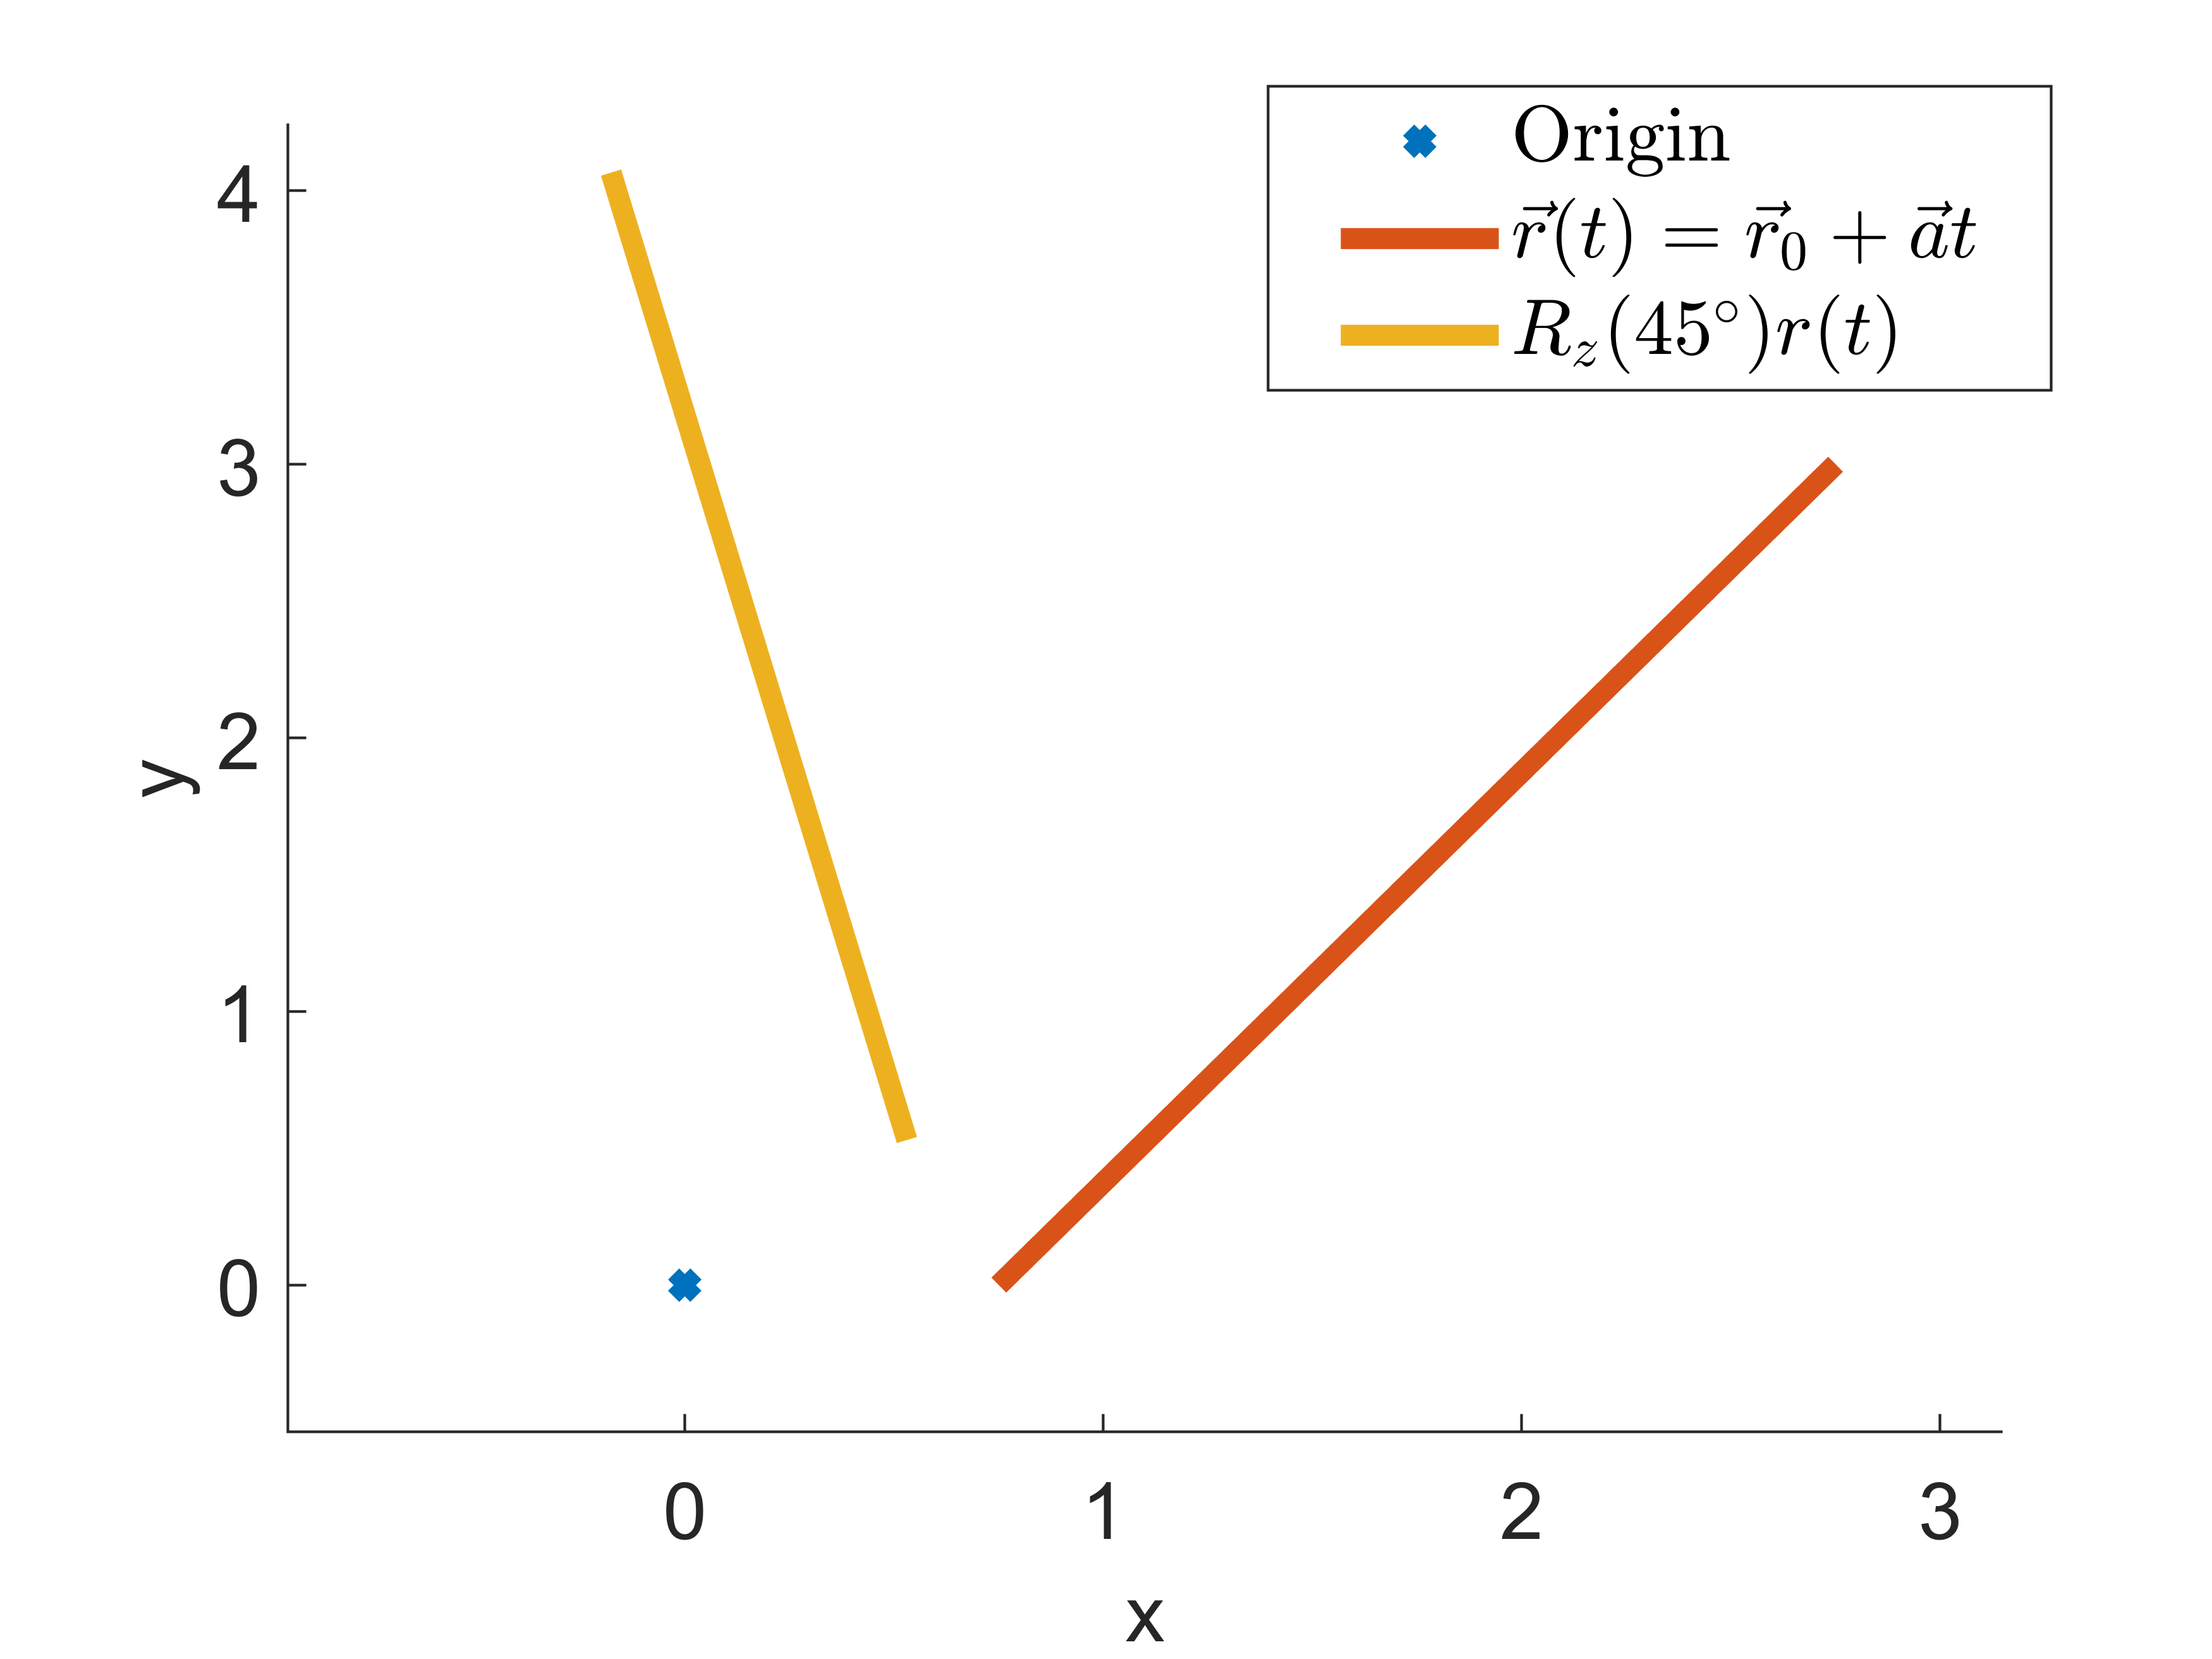
\includegraphics[height=4.6cm,width=1\textwidth,keepaspectratio]{line_example.png}
                % \caption*{\footnotesize $r(t)=\begin{bmatrix}\frac{3}{4}\\0\end{bmatrix}+\begin{bmatrix}2\\3\end{bmatrix}t$}
                \label{fig:line_example.png}
            \end{figure}
        \end{column}
    \end{columns}

\end{frame}

\begin{frame}[t]{Segment line in parametric form}
\framesubtitle{}
    \begin{columns}[T,onlytextwidth]
        \begin{column}{0.49\textwidth}
            AGLA (6th lab) --- $\vec{r}(t)=\vec{p}_0+a(t)$ or \\ $\left\{\begin{matrix*}[l]
            x = p_{0x} + a_x t\\ 
            y = p_{0y} + a_y t\\
            z = p_{0z} + a_z t
            \end{matrix*}\right.$

        {Not easy to make a segment line (we have only one clear point and a direction)}
        \end{column}
        \begin{column}{0.49\textwidth}
            $\vec{r}(t)=\vec{p}_0(1-t)+\vec{p}_1 t$ or $\left\{\begin{matrix*}[l]
                x = p_{0x}(1-t) + p_{1x} t\\ 
                y = p_{0y}(1-t) + p_{1y} t\\
                z = p_{0z}(1-t) + p_{1z} t
                \end{matrix*}\right.$

                {It is really convenient, if you know 2 points and want to make a segment line. We will meet this form a lof of times today}
        \end{column}
    \end{columns}
\end{frame}

\begin{frame}[t]{Polyline (Polygonal chain)}
\framesubtitle{}
    \begin{columns}[T,onlytextwidth]
        \begin{column}{0.49\textwidth}
            $\vec{r}(t)=\vec{p}_i(1-w)+\vec{p}_{i+1}w$, where $w$ is a local parameter $w=\dfrac{t-t_i}{t_{t+1}-t_i}$, $t_i \leq t \leq t_{i+1}$

            Polyline passes through given control points $\vec{p}_0,\ \vec{p}_1, ..., \vec{p}_n$. $t_i \leq t_{i+1}$

            \textbf{Example}
            $\vec{p}_0 = \begin{bmatrix} 2\\ 0 \end{bmatrix},\ \vec{p}_1 = \begin{bmatrix} 4\\ 2 \end{bmatrix},\ \vec{p}_2 = \begin{bmatrix} 7\\ 2 \end{bmatrix},\ \vec{p}_3 = \begin{bmatrix} 6\\ 0 \end{bmatrix}$
        \end{column}
        \begin{column}{0.49\textwidth}
            If each knot will be the same and equal to 1, then  $\vec{r}(t)=\vec{p}_i(1-t)+\vec{p}_{i+1} t$, $i=0...n-1$
                \begin{figure}[H]
                    \centering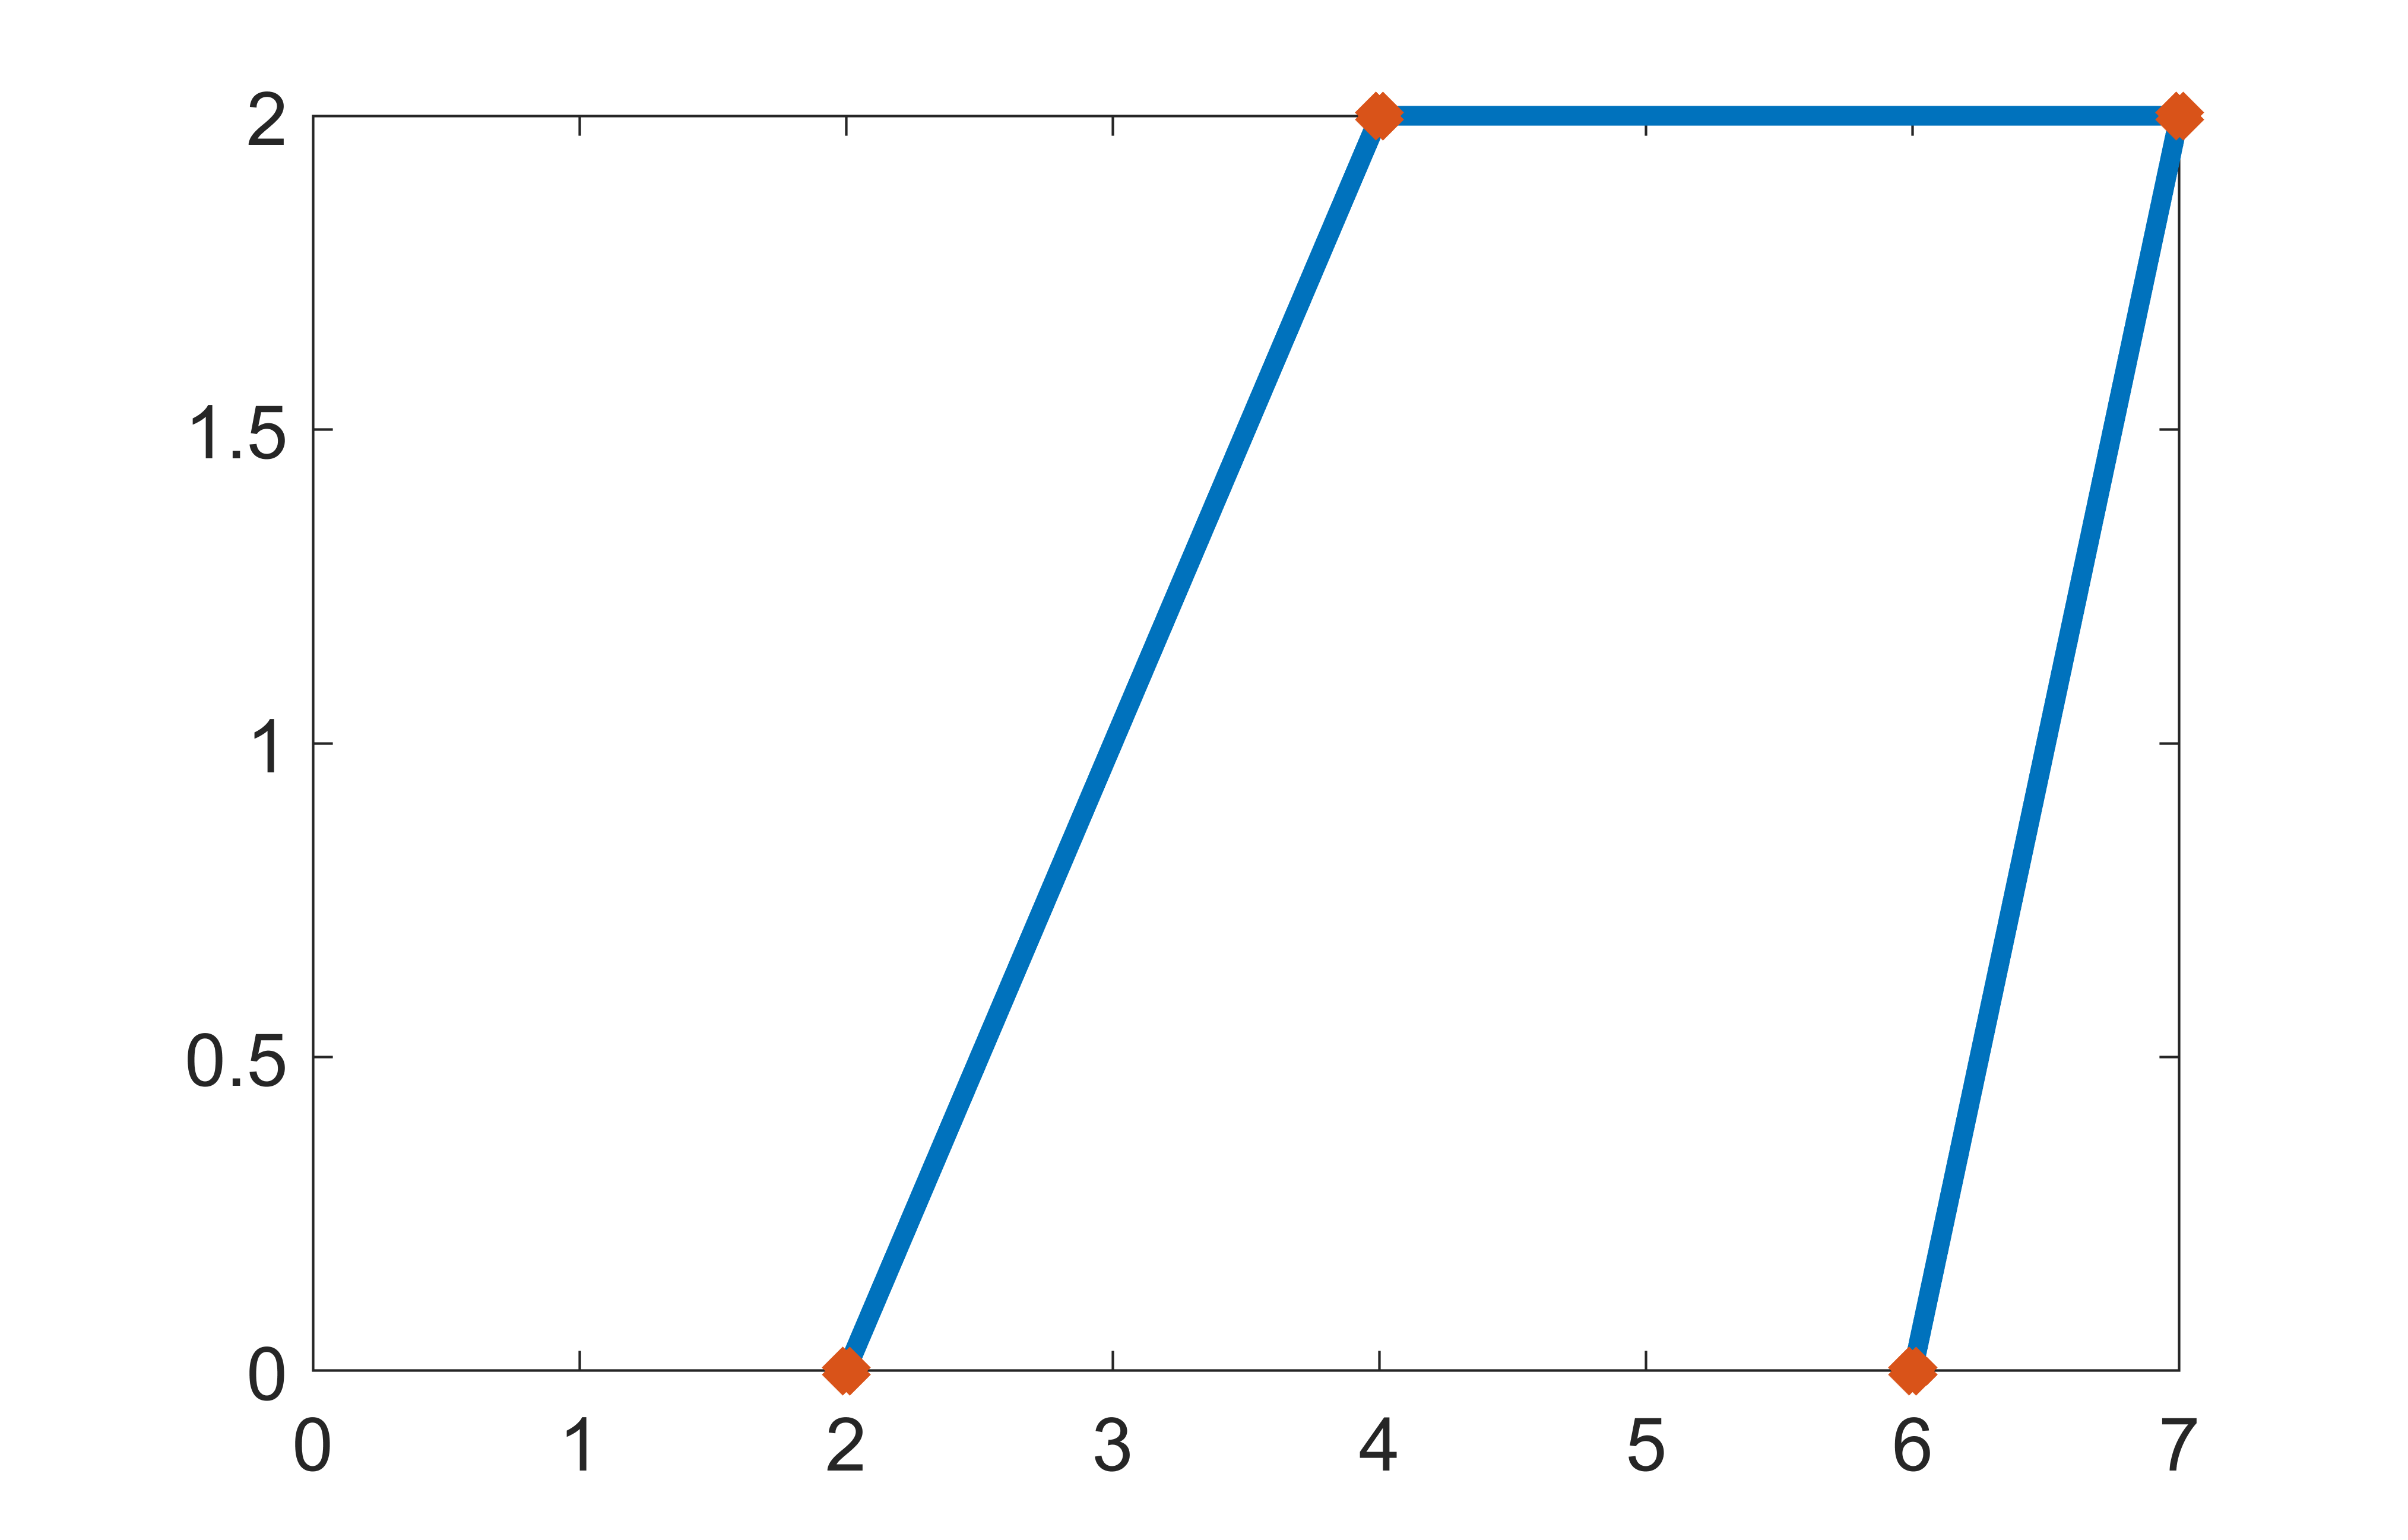
\includegraphics[height=5cm,width=1\textwidth,keepaspectratio]{polyline_concrete.png}
                    % \caption{caption_name}
                    \label{fig:polyline_concrete.png}
                \end{figure}
        \end{column}
    \end{columns}
\end{frame}

\begin{frame}[t]{Intro to splines}
    \framesubtitle{Video}
    \vspace{-0.6cm}
    \begin{figure}[H]
        \href{https://youtu.be/aVwxzDHniEw}{
            \centering
\includegraphics[height=6cm,width=1\textwidth,keepaspectratio]{beauty_of_bezier_video.jpg}}
        % \caption{Click on a picture for a video}
        \label{fig:beauty_of_bezier_video.jpg}
    \end{figure}
\end{frame}

\begin{frame}[t]{Splines}
\framesubtitle{Informal Definition}
    \begin{columns}[T,onlytextwidth]
        \begin{column}{0.39\textwidth}
            \textbf{Splines} (\textit{piecewise polynomial} functions) are awesome tool to construct \textit{smooth} and flexible shapes in computer graphics.
        \end{column}
        \begin{column}{0.59\textwidth}
            \vspace{-1cm}
            \begin{figure}[H]
                \begin{subfigure}[b]{0.49\textwidth}
                    \centering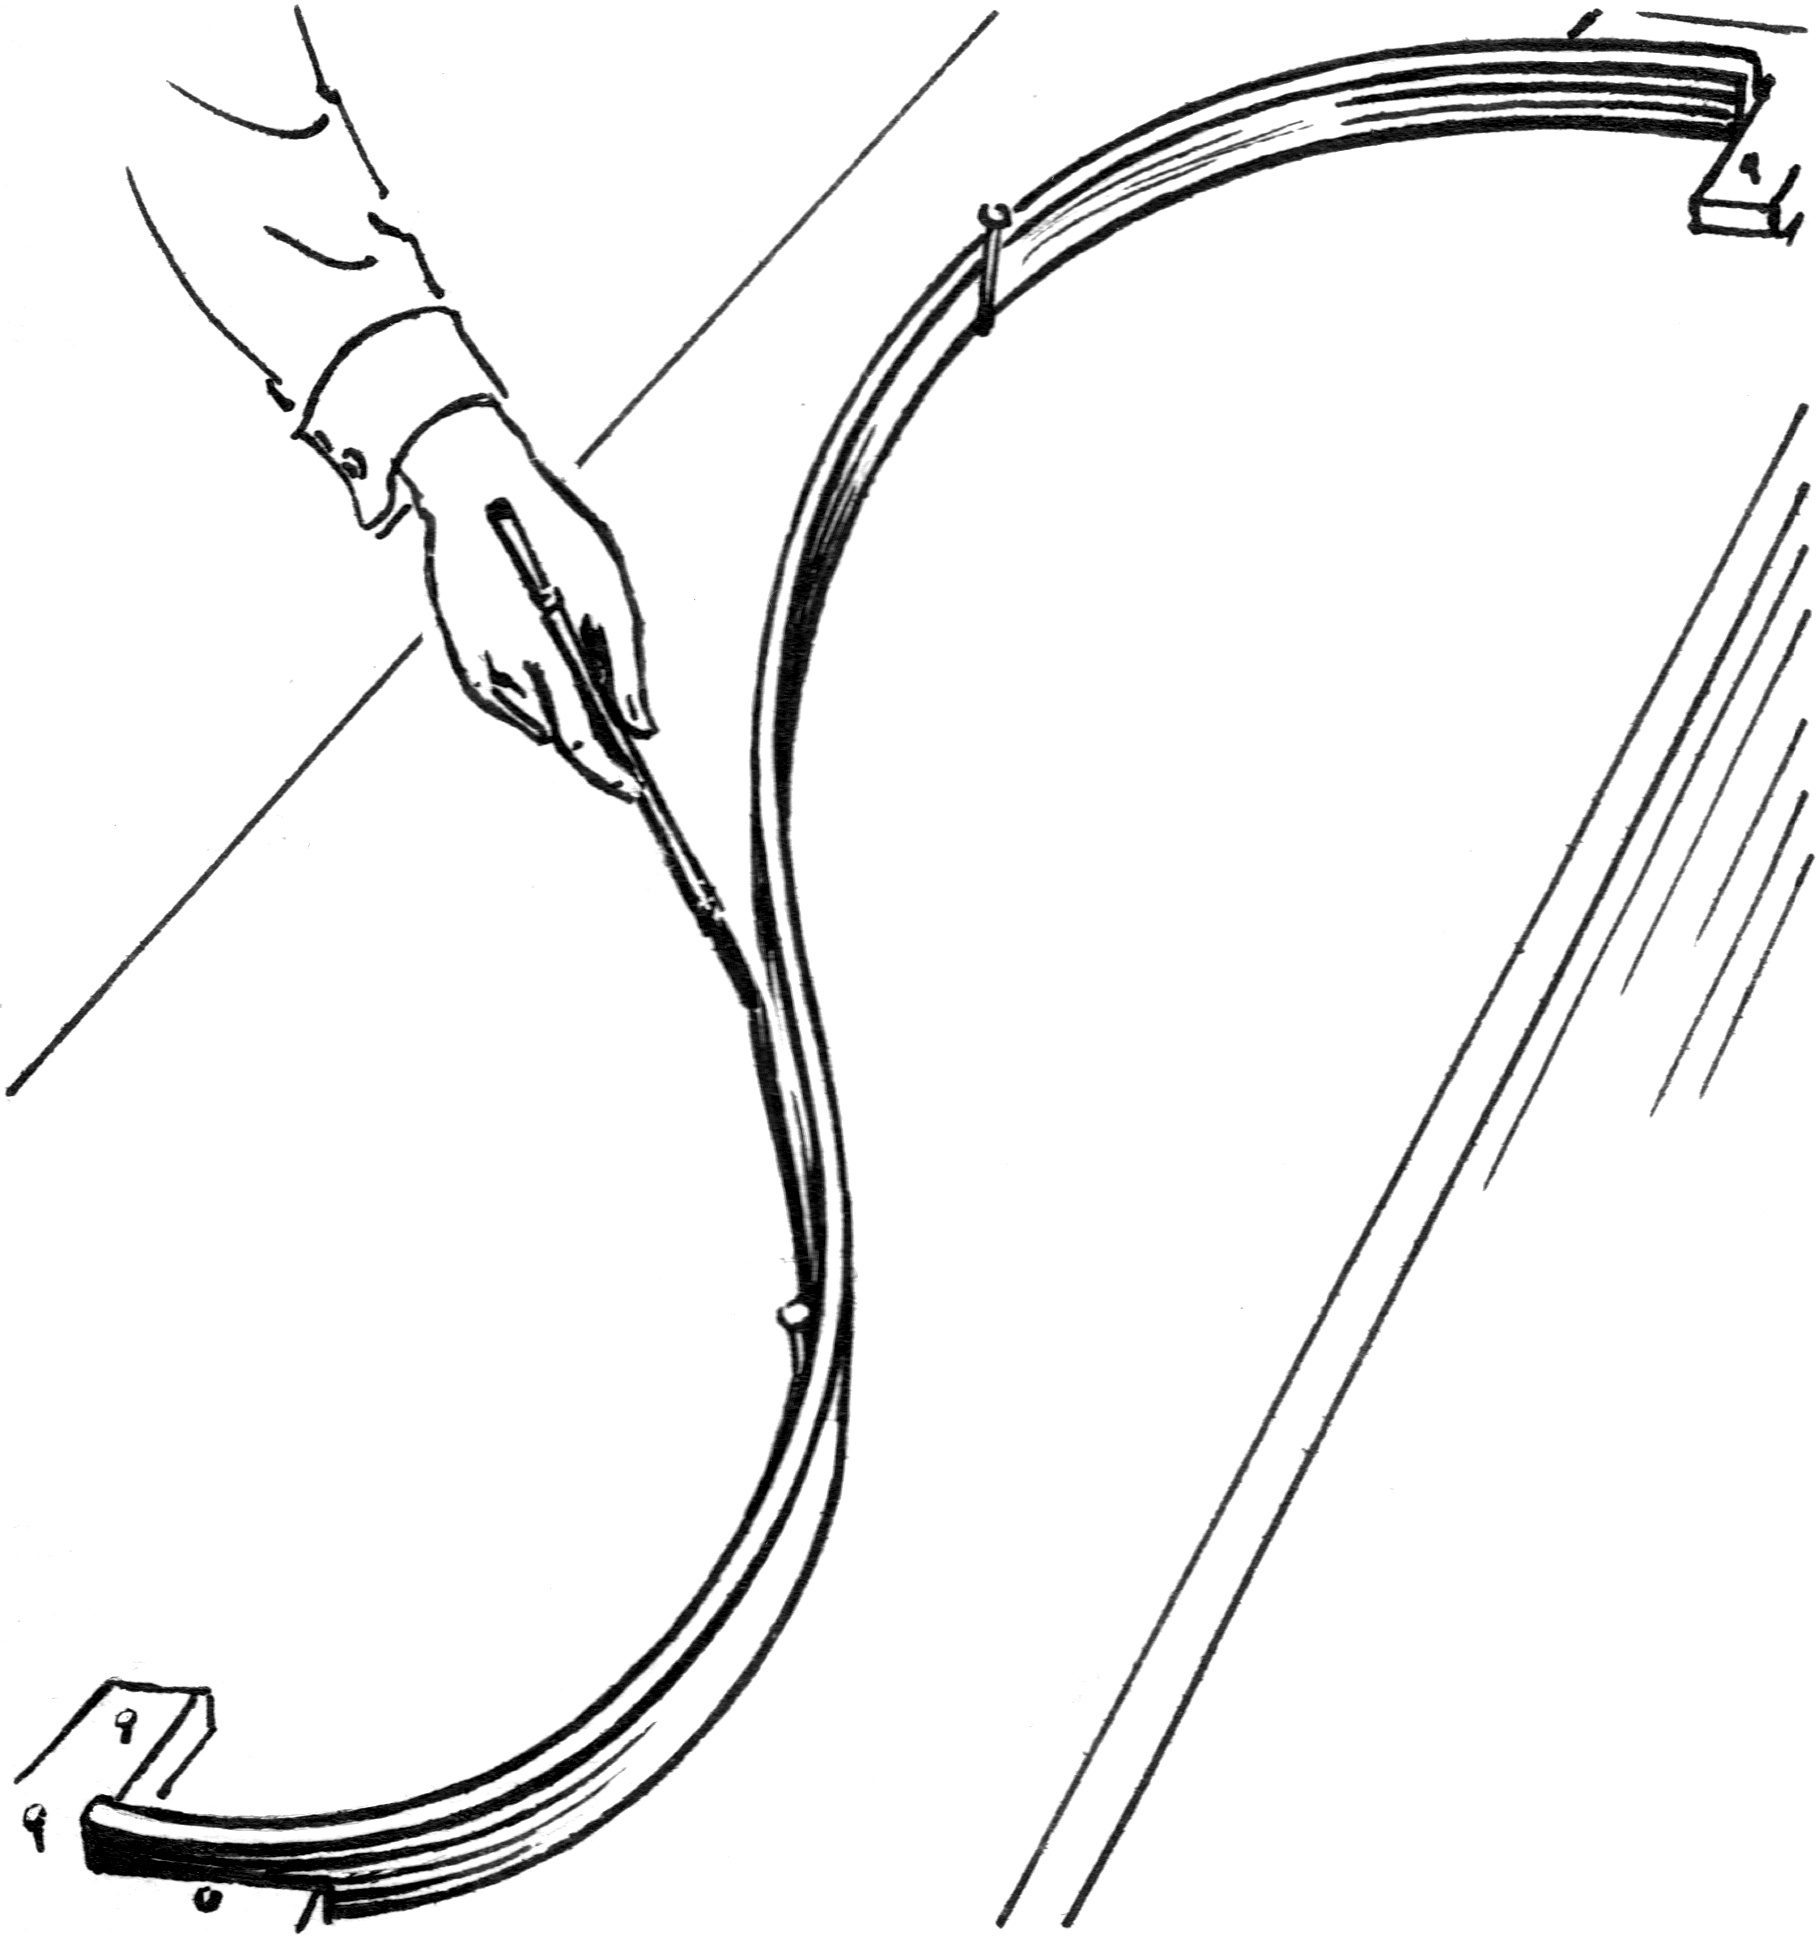
\includegraphics[height=5cm,width=1\textwidth,keepaspectratio]{spline_ship.png}
                    \caption*{Starting 15th century, ship hull designers used splines for making a smooth shape}
                    \label{fig:spline_ship.png}
                \end{subfigure}
                \begin{subfigure}[b]{0.49\textwidth}
                    \centering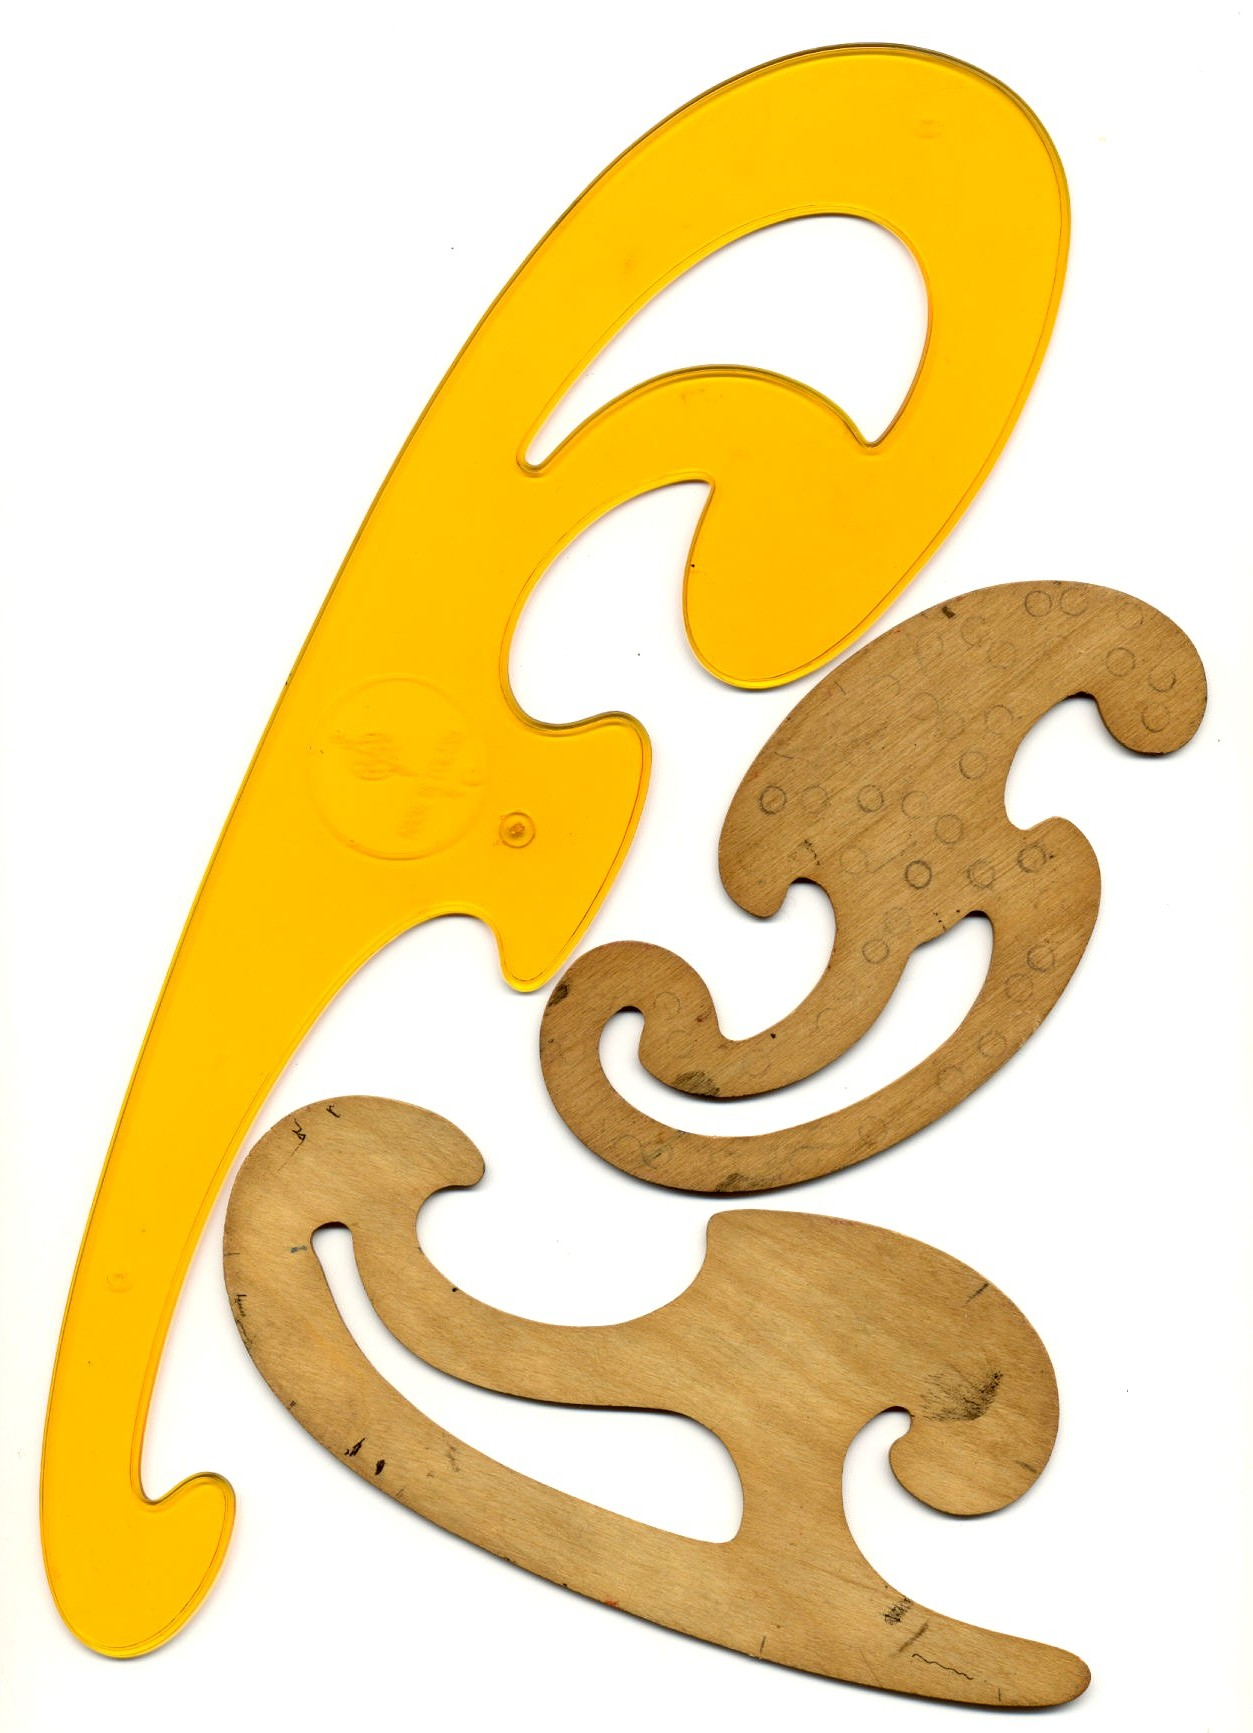
\includegraphics[height=5cm,width=1\textwidth,keepaspectratio]{lekalo.jpg}
                    \caption*{French curve (Лекало)}
                    \label{fig:lekalo.jpg}
                \end{subfigure}
            \end{figure}
        \end{column}
    \end{columns}
\end{frame}

\begin{frame}[t]{Splines: Applications}
% \framesubtitle{Applications}
\vspace{-0.6cm}
    \begin{figure}[H]
        \begin{subfigure}[t]{0.32\textwidth}
            \centering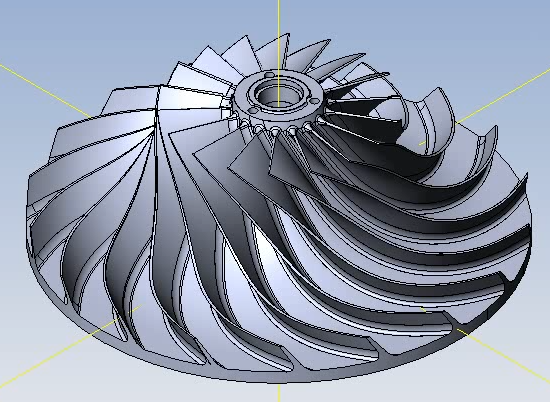
\includegraphics[height=2.4cm,width=1\textwidth,keepaspectratio]{lopatka.png}
            \caption*{User: Car shape design, aircrafting}
        \end{subfigure}
        \begin{subfigure}[t]{0.32\textwidth}
            \centering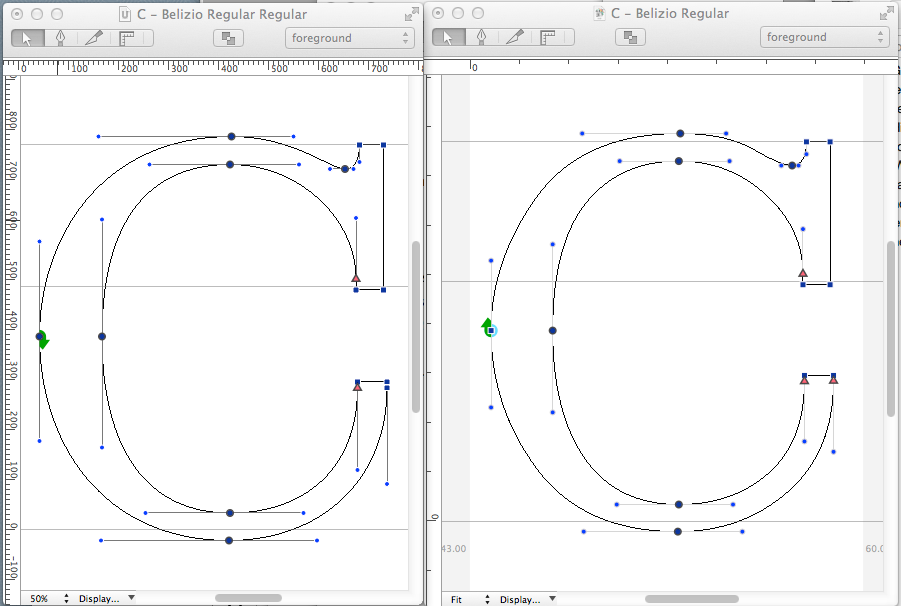
\includegraphics[height=2.4cm,width=1\textwidth,keepaspectratio]{font_creation.png}
            \caption*{User: Make fonts}
        \end{subfigure}
        \begin{subfigure}[t]{0.32\textwidth}
            \centering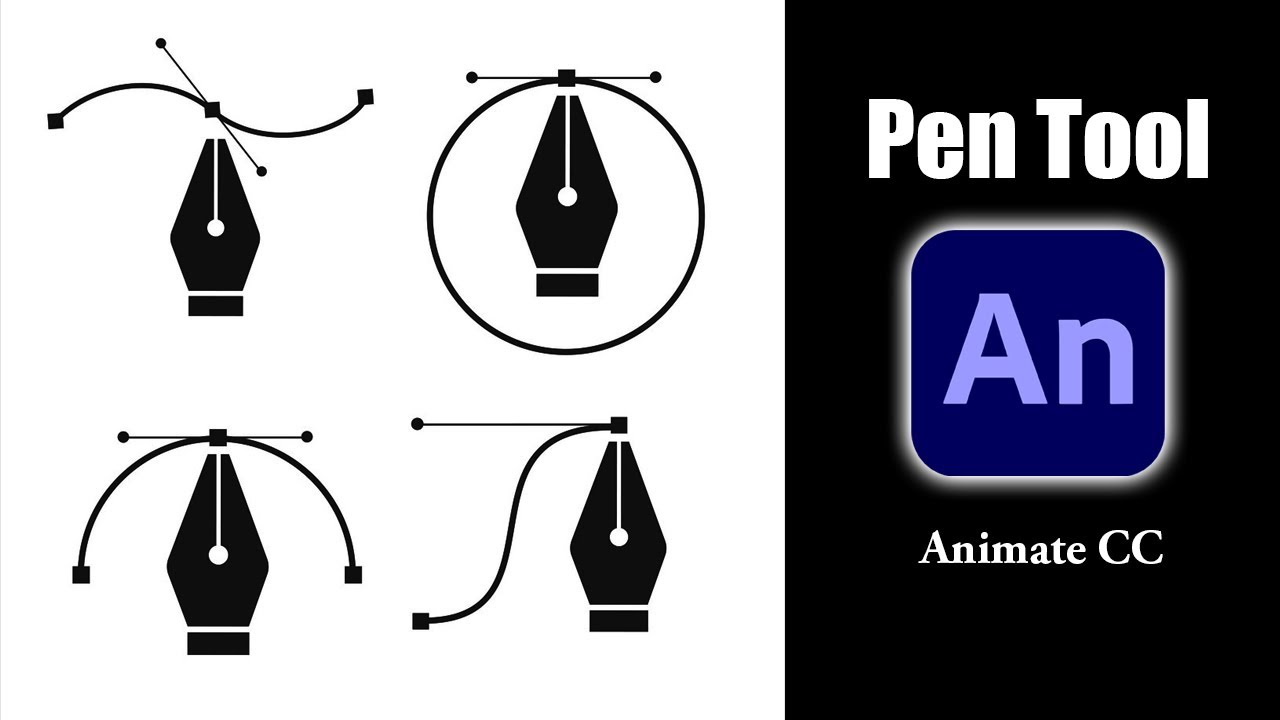
\includegraphics[height=2.4cm,width=1\textwidth,keepaspectratio]{pen_tool.jpg}
            \caption*{User: Pen tool in PhotoShop}
        \end{subfigure}

        \begin{subfigure}[t]{0.32\textwidth}
            \centering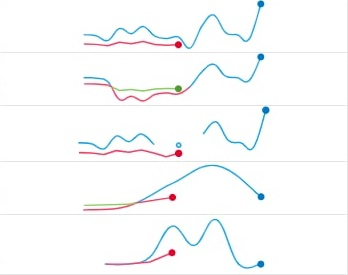
\includegraphics[height=2.5cm,width=1\textwidth,keepaspectratio]{multi_splines_interpolation.jpg}
            \caption*{Math: Interpolation --- advanced data analysis }
        \end{subfigure}
        \begin{subfigure}[t]{0.32\textwidth}
            \centering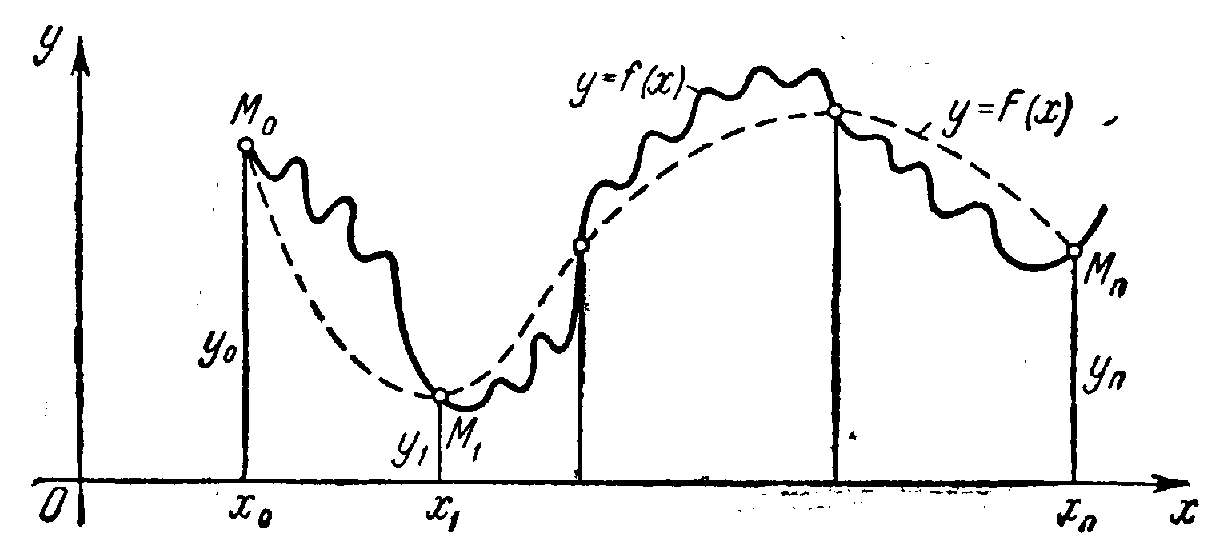
\includegraphics[height=2.5cm,width=1\textwidth,keepaspectratio]{spline_noise_reduction.png}
            \caption*{Math: Approximation --- signal post processing (reduce noise)}
        \end{subfigure}
        \begin{subfigure}[t]{0.32\textwidth}
            \centering
\includegraphics[height=2.5cm,width=1\textwidth,keepaspectratio]{stonks.jpg}
            \caption*{Math: Extrapolation --- revenue prediction during the covid}
        \end{subfigure}
    
    \end{figure}
\end{frame}

\note{
    \footnotesize
    Использовал сплайны при прогнозировании выручки во время ковида: был бейзлайн прогноз, на который я умножал на кривую (сигмоиду), которую рассчитывал в соответствии с последними точками факта. Часть параметров кривой была зафиксирована, а часть обновлялась каждый день.
Так мы получили более-менее точный прогноз во время кризиса.

Ну вот тут интерполяция, да. У тебя есть набор точек, но для красивого графика ты рассчитываешь промежуточные точки.

Ну приходят тебе дискретные сигналы с датчика, ты восстанавливаешь функцию, вот чтобы эта функция была похожа на реальность надо юзать сплайн
}

\begin{frame}[t]{Cubic spline}
\framesubtitle{}
\begin{align*}
    \vec{r}(t) = (1-w)\vec{p}_0 + w\vec{p}_{i+1} + ((-2w+3w^2-w^3)\vec{s}_i+(-w+w^3)\vec{s}_{i+1})\dfrac{(t_{i+1}-t_i)^2}{6},
\end{align*}
    \begin{columns}[T,onlytextwidth]
        \begin{column}{0.49\textwidth}
            \begin{align*}
                w=\dfrac{t-t_i}{t_{t+1}-t_i},\ t_i \leq t \leq t_{i+1} \\
                s_i \text{ --- second derivative in control points} \\ 
                s_0 = s_n = 0
            \end{align*}
        \end{column}
        \begin{column}{0.49\textwidth}
            \begin{figure}[H]
                \centering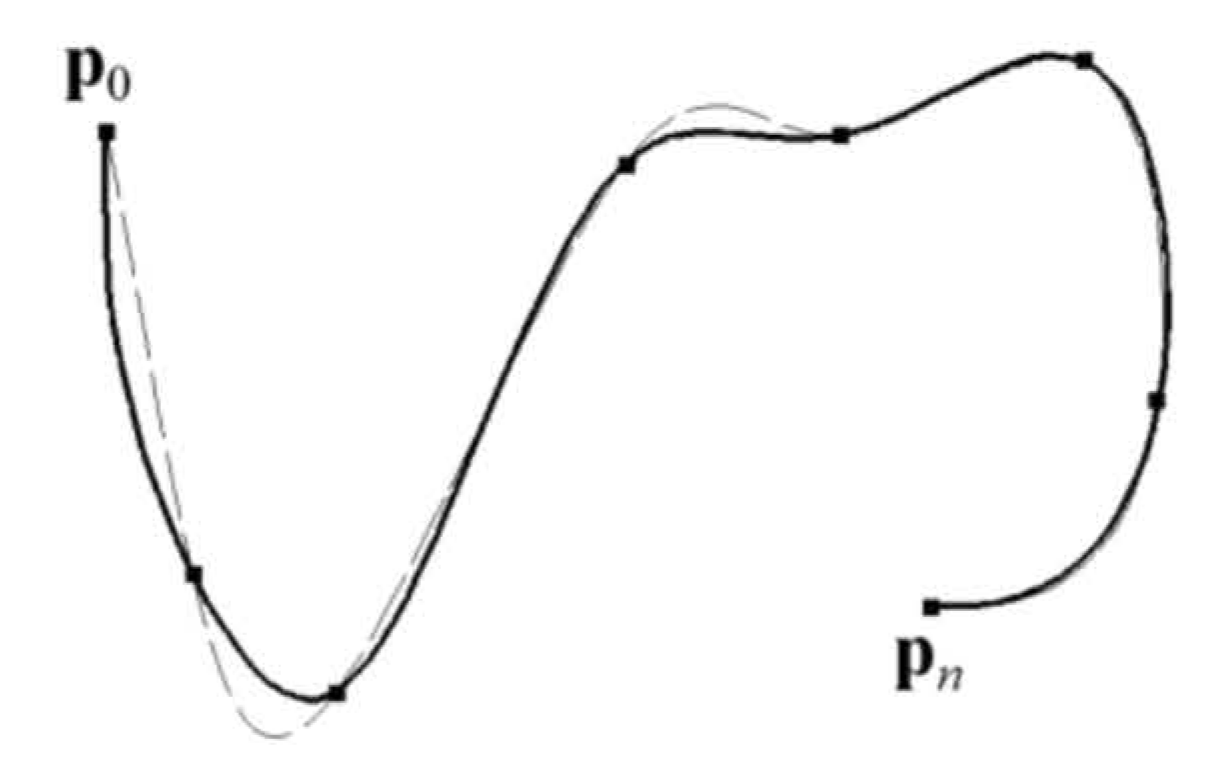
\includegraphics[height=4cm,width=1\textwidth,keepaspectratio]{cubic_spline_book.png}
                % \caption{caption_name}
                \label{fig:cubic_spline_book.png}
            \end{figure} 
        \end{column}
    \end{columns}
\end{frame}

\begin{frame}[t]{Cubic spline in Fusion 360}
    \framesubtitle{Video}
    \vspace{-0.6cm}
    \begin{figure}[H]
        \href{run:./videos/cubic_spline_video.mp4}{
            \centering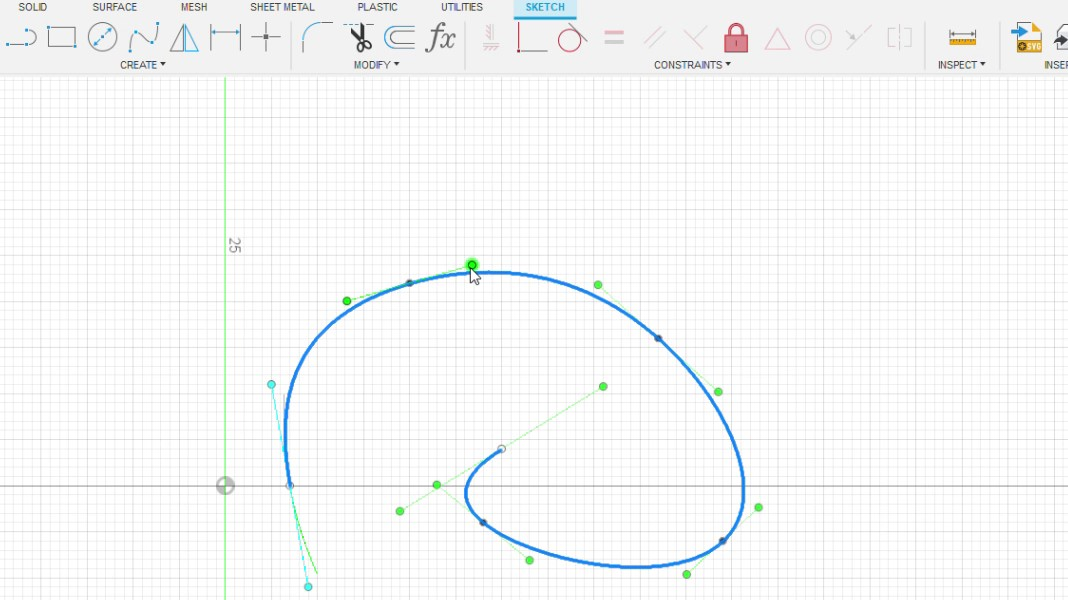
\includegraphics[height=6cm,width=1\textwidth,keepaspectratio]{cubic_spline_video_preview.jpg}}
        % \caption{Click on a picture for a video}
    \end{figure}
\end{frame}

\begin{frame}[t]{Bezier spline}
\framesubtitle{}
    \begin{columns}[T,onlytextwidth]
        \begin{column}{0.59\textwidth}
            1-st order curve
            \begin{align*}
                \vec{r}(t)=(1-t)\vec{p}_{0}+t\vec{p}_{1}
            \end{align*}
            2-nd order curve
            \begin{align*}
                \vec{r}(t)=(1-t)^{2}\vec{p}_{0}+2t(1-t)\vec{p}_{1}+t^{2}\vec{p}_{2}
            \end{align*}
            General form
            \begin{align*}
                \vec{r}(t) = \sum_{i=0}^{n} B_i^n(t)\vec{p}_i
            \end{align*}
            \begin{align*}
                B_i^n(t) = \frac{n!}{i!(n-i)!}t^i(1-t)^{n-i} \text{Bernstein polynomials}
            \end{align*}
        \end{column}
        \begin{column}{0.39\textwidth}
            \vspace{-1cm}
            \begin{figure}[H]
                \centering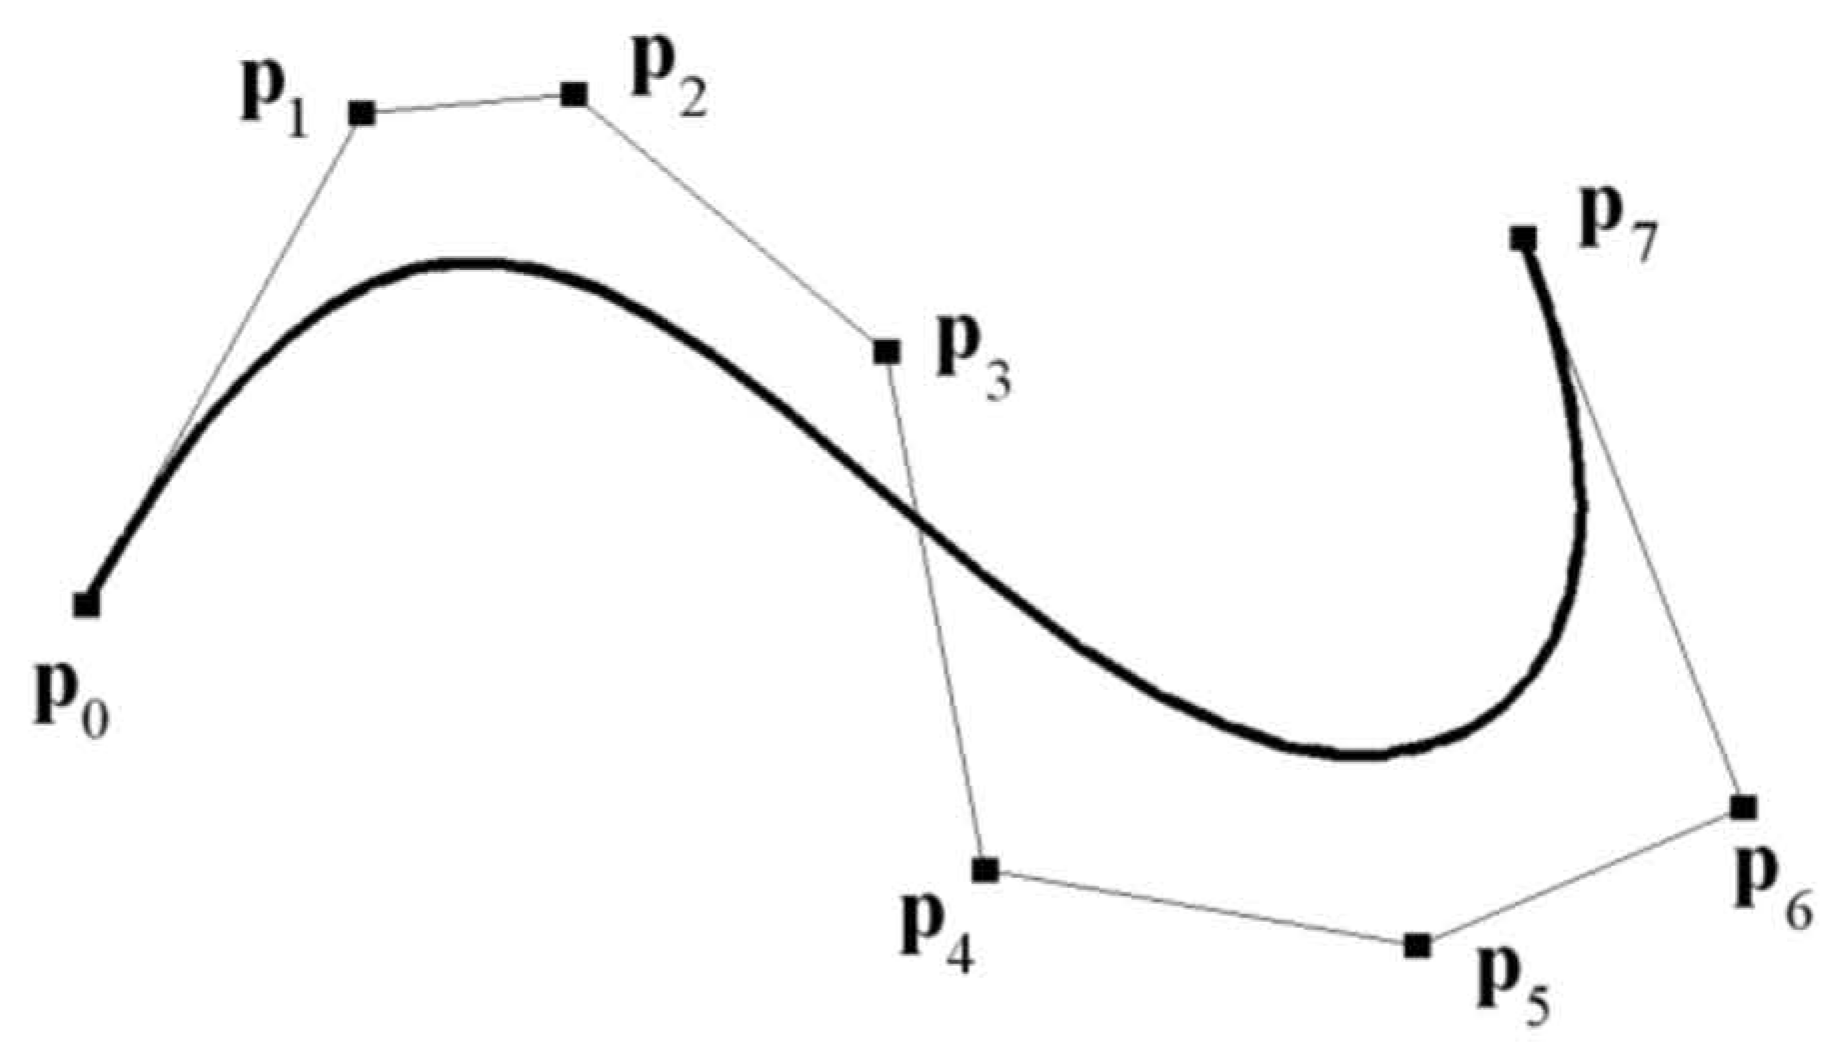
\includegraphics[height=2.5cm,width=1\textwidth,keepaspectratio]{bezier_spline_book.png}
                % \caption{caption_name}
                \label{fig:bezier_spline_book.png}
            \end{figure}
            \begin{figure}[H]
                \href{run:./videos/bezier_big.gif}{
                    \centering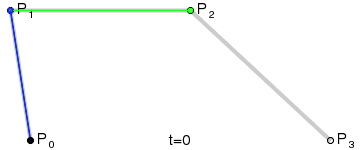
\includegraphics[height=2.5cm,width=1\textwidth,keepaspectratio]{bezier_big.png}}
                % \caption{Click on a picture for a video}
            \end{figure}
        \end{column}
    \end{columns}
\end{frame}

\begin{frame}[t]{Bezier spline in Fusion 360}
    \framesubtitle{Video}
    \vspace{-0.6cm}
    \begin{figure}[H]
        \href{run:./videos/bezier_spline_video.mp4}{
            \centering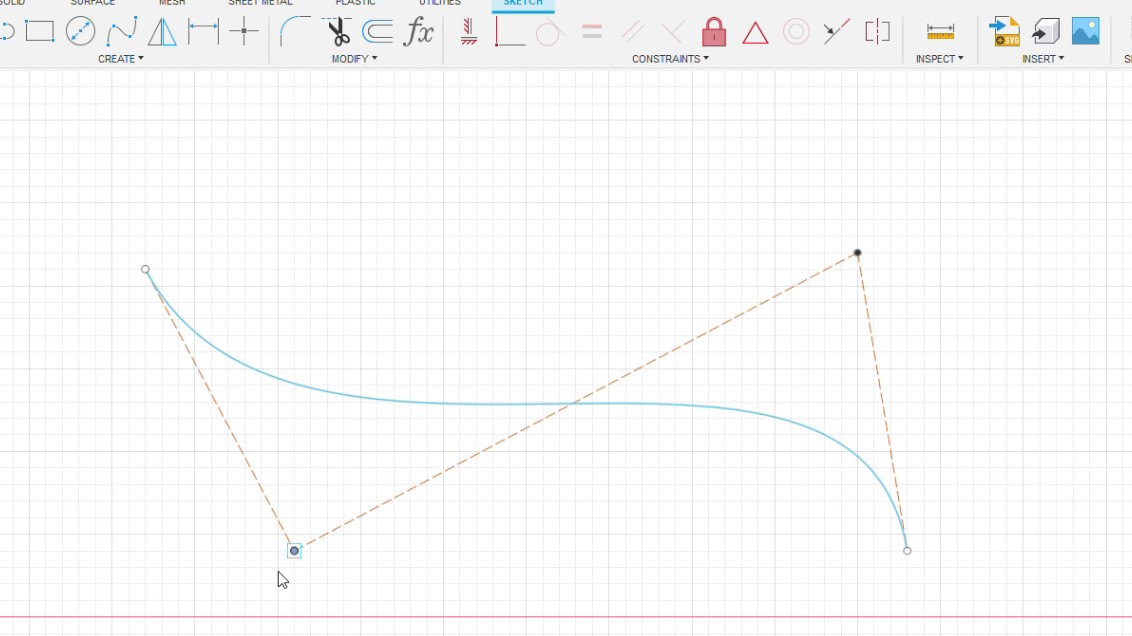
\includegraphics[height=6cm,width=1\textwidth,keepaspectratio]{bezier_spline_video_preview.jpg}}
        % \caption{Click on a picture for a video}
    \end{figure}
\end{frame}

\begin{frame}[t]{Relationship between splines and conic sections (1)}
\framesubtitle{}
\vspace{-0.5cm}
            \begin{figure}[H]
                \centering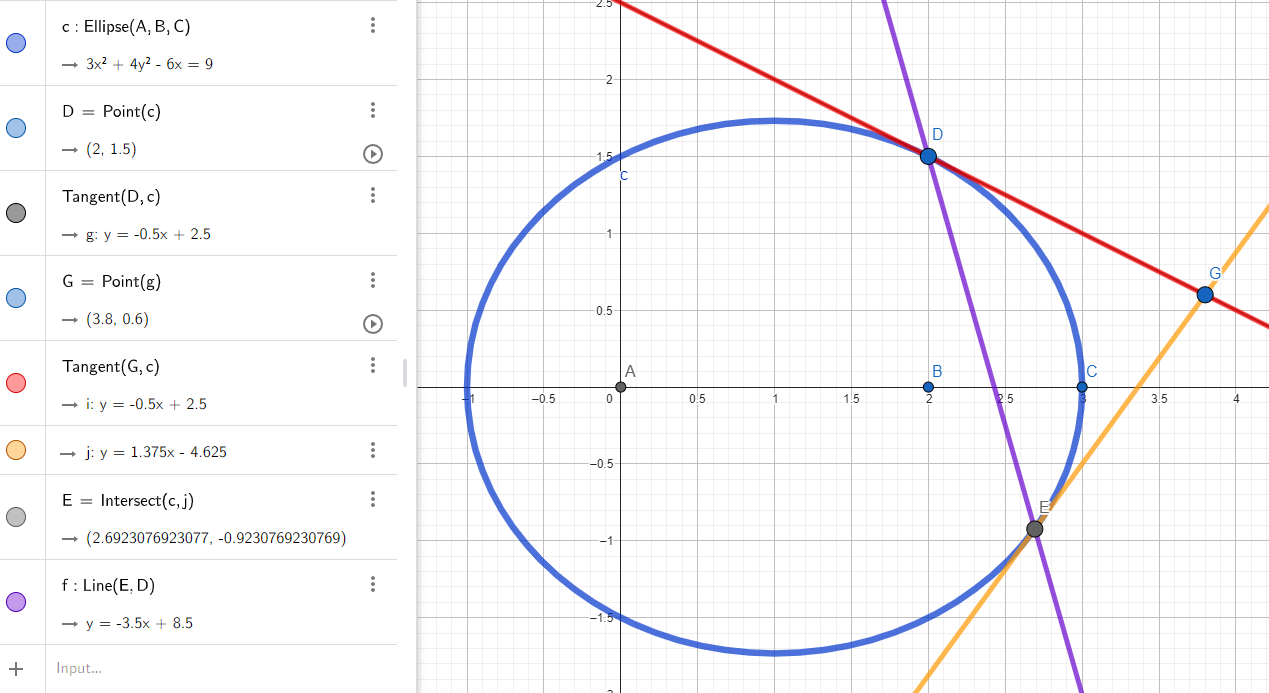
\includegraphics[height=6.5cm,width=1\textwidth,keepaspectratio]{bezier_to_conic_intro.png}
                % \caption{caption_name}
                \label{fig:bezier_to_conic_intro.png}
            \end{figure}
\end{frame}

\begin{frame}[t]{Relationship between splines and conic sections (2)}
    \framesubtitle{}
    \vspace{-0.5cm}
        \begin{figure}[H]
            \centering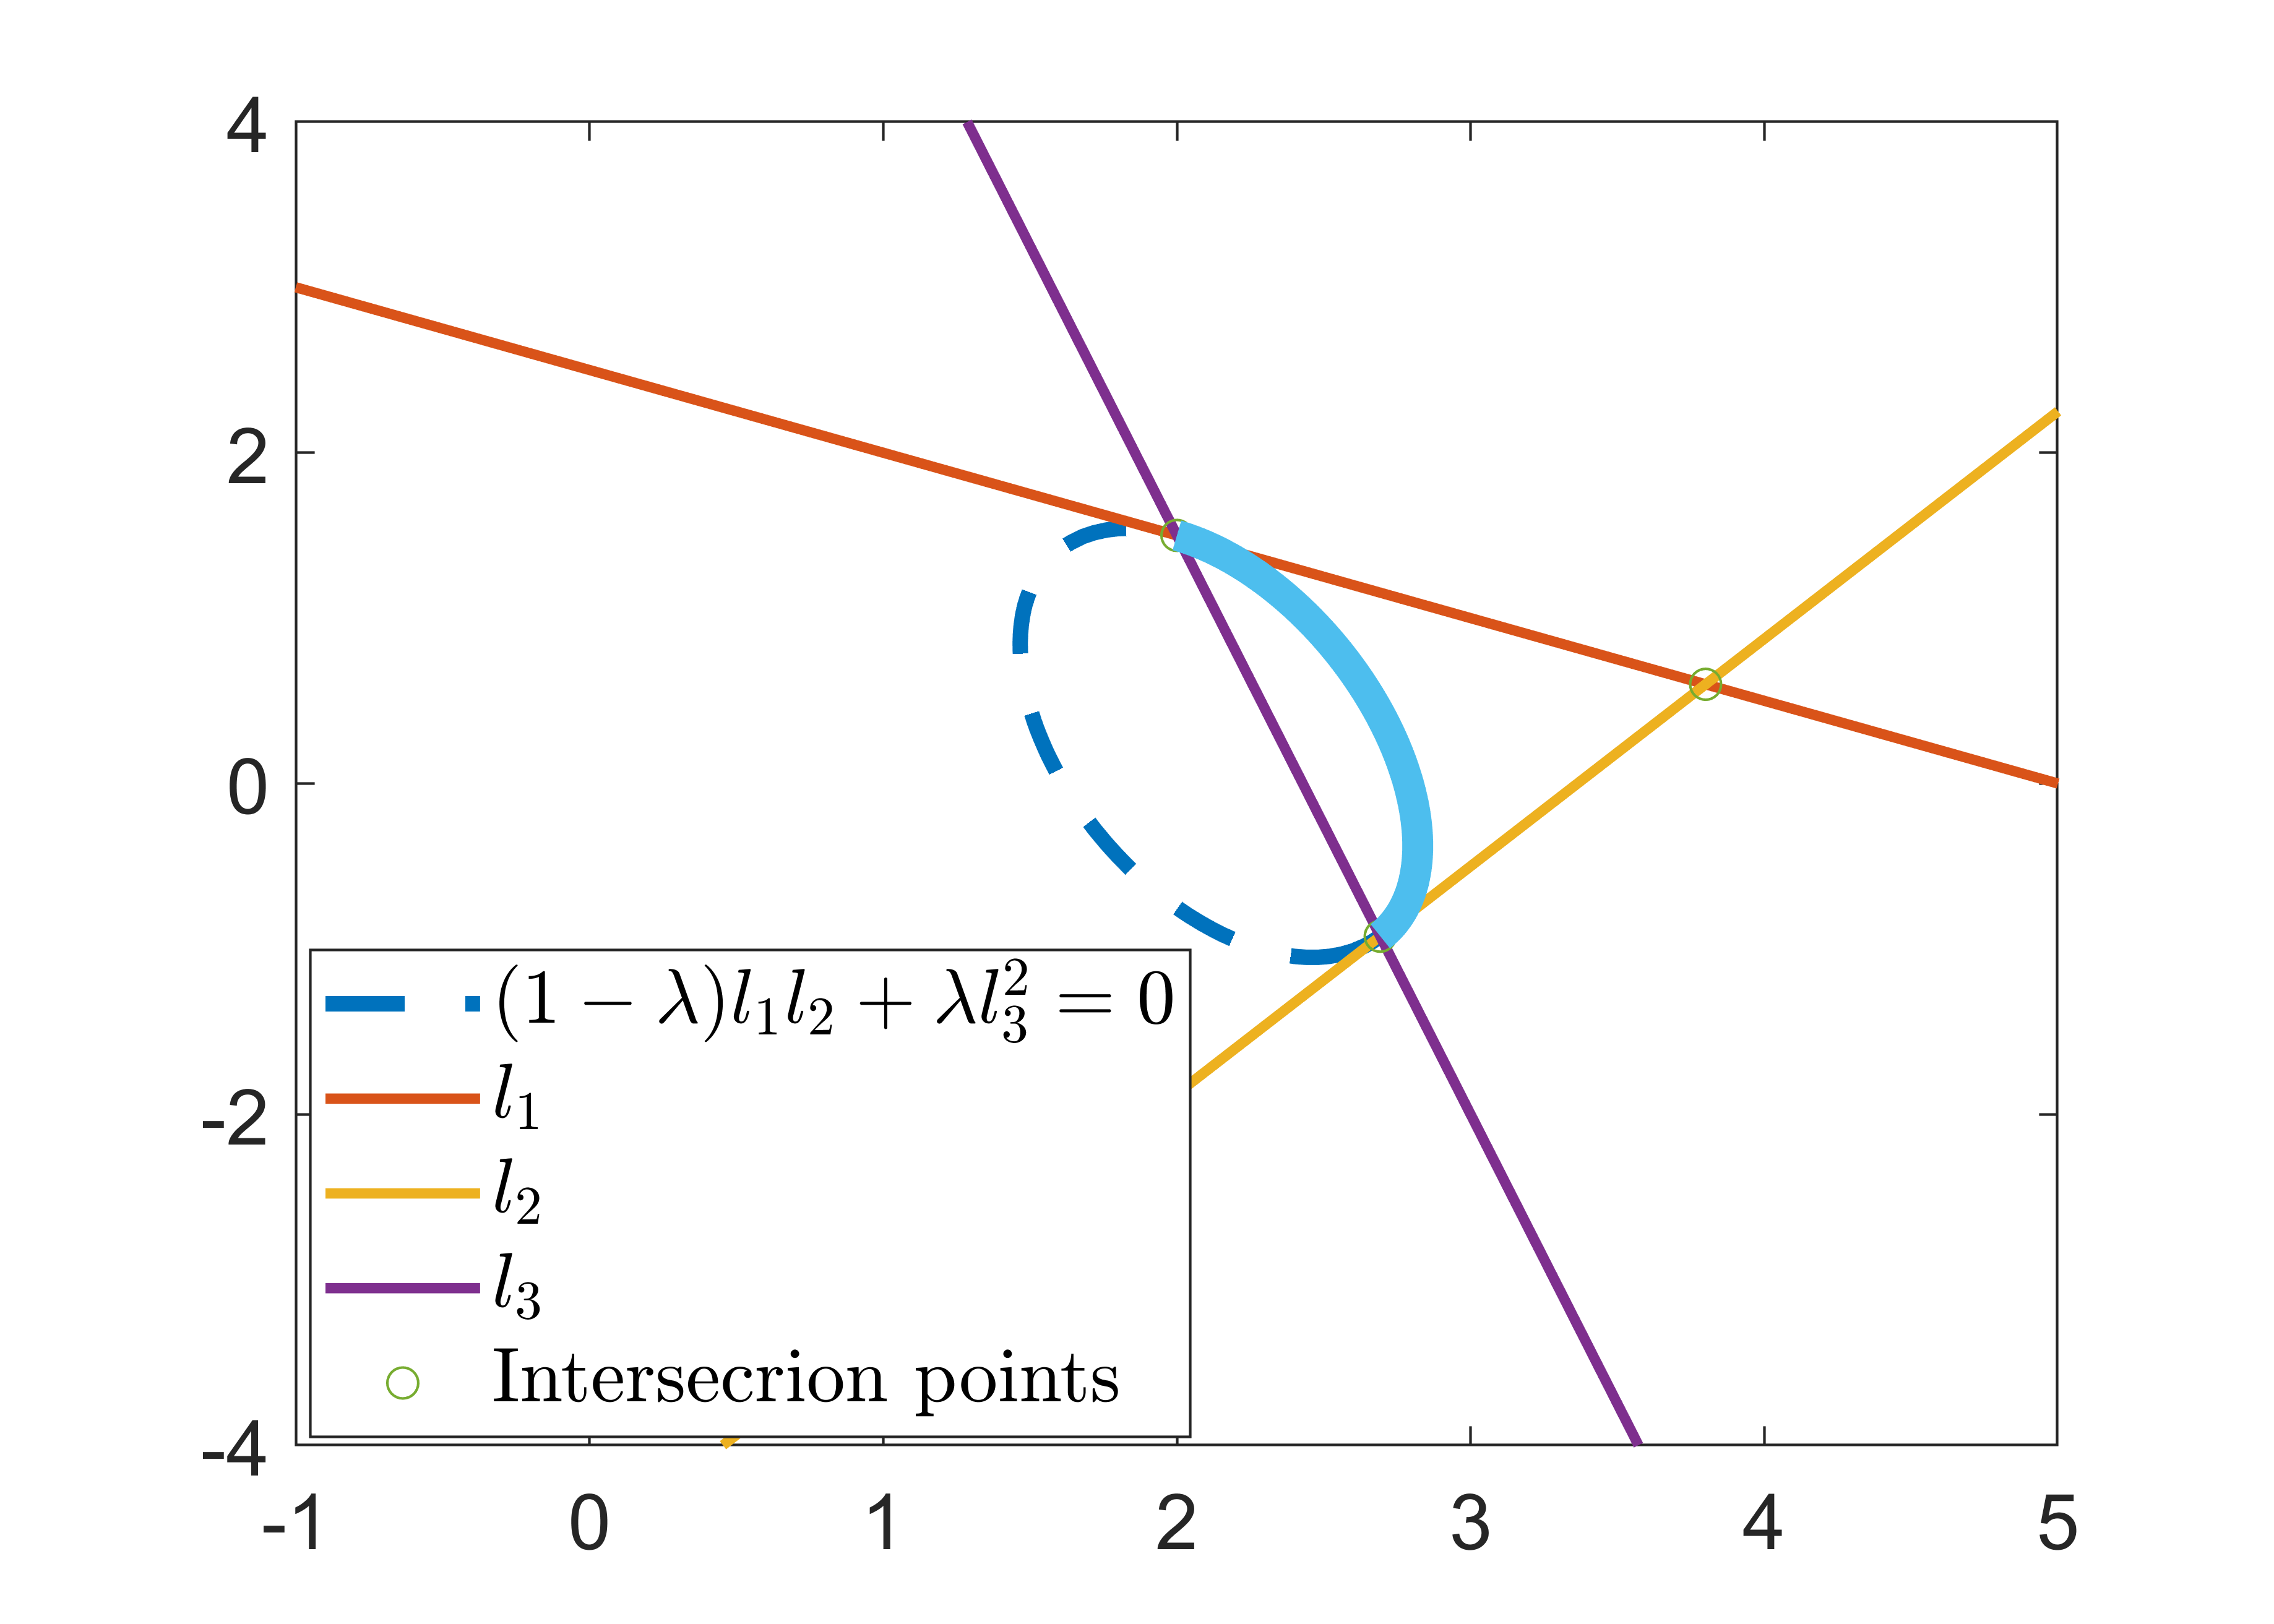
\includegraphics[height=6.5cm,width=1\textwidth,keepaspectratio]{bezier_to_conic.png}
            % \caption{caption_name}
            \label{fig:bezier_to_conic.png}
        \end{figure}
    \end{frame}

\begin{frame}[t]{Surface made by extruding and sweeping}
\framesubtitle{}
    \begin{columns}[T,onlytextwidth]
        \begin{column}{0.49\textwidth}
            When a generating curve moves along a guiding curve, the orientation of the generating curve may remain unchanged related to guiding line. 
            
            If the guiding line is a straight line --- \textbf{extruding surface}, otherwise --- \textbf{sweeping surface}
            \begin{align*}
                \vec{r}(u,v) = \vec{c}(u) + \vec{d}v
            \end{align*}
        \end{column}
        \begin{column}{0.49\textwidth}
            \begin{figure}[H]
                \centering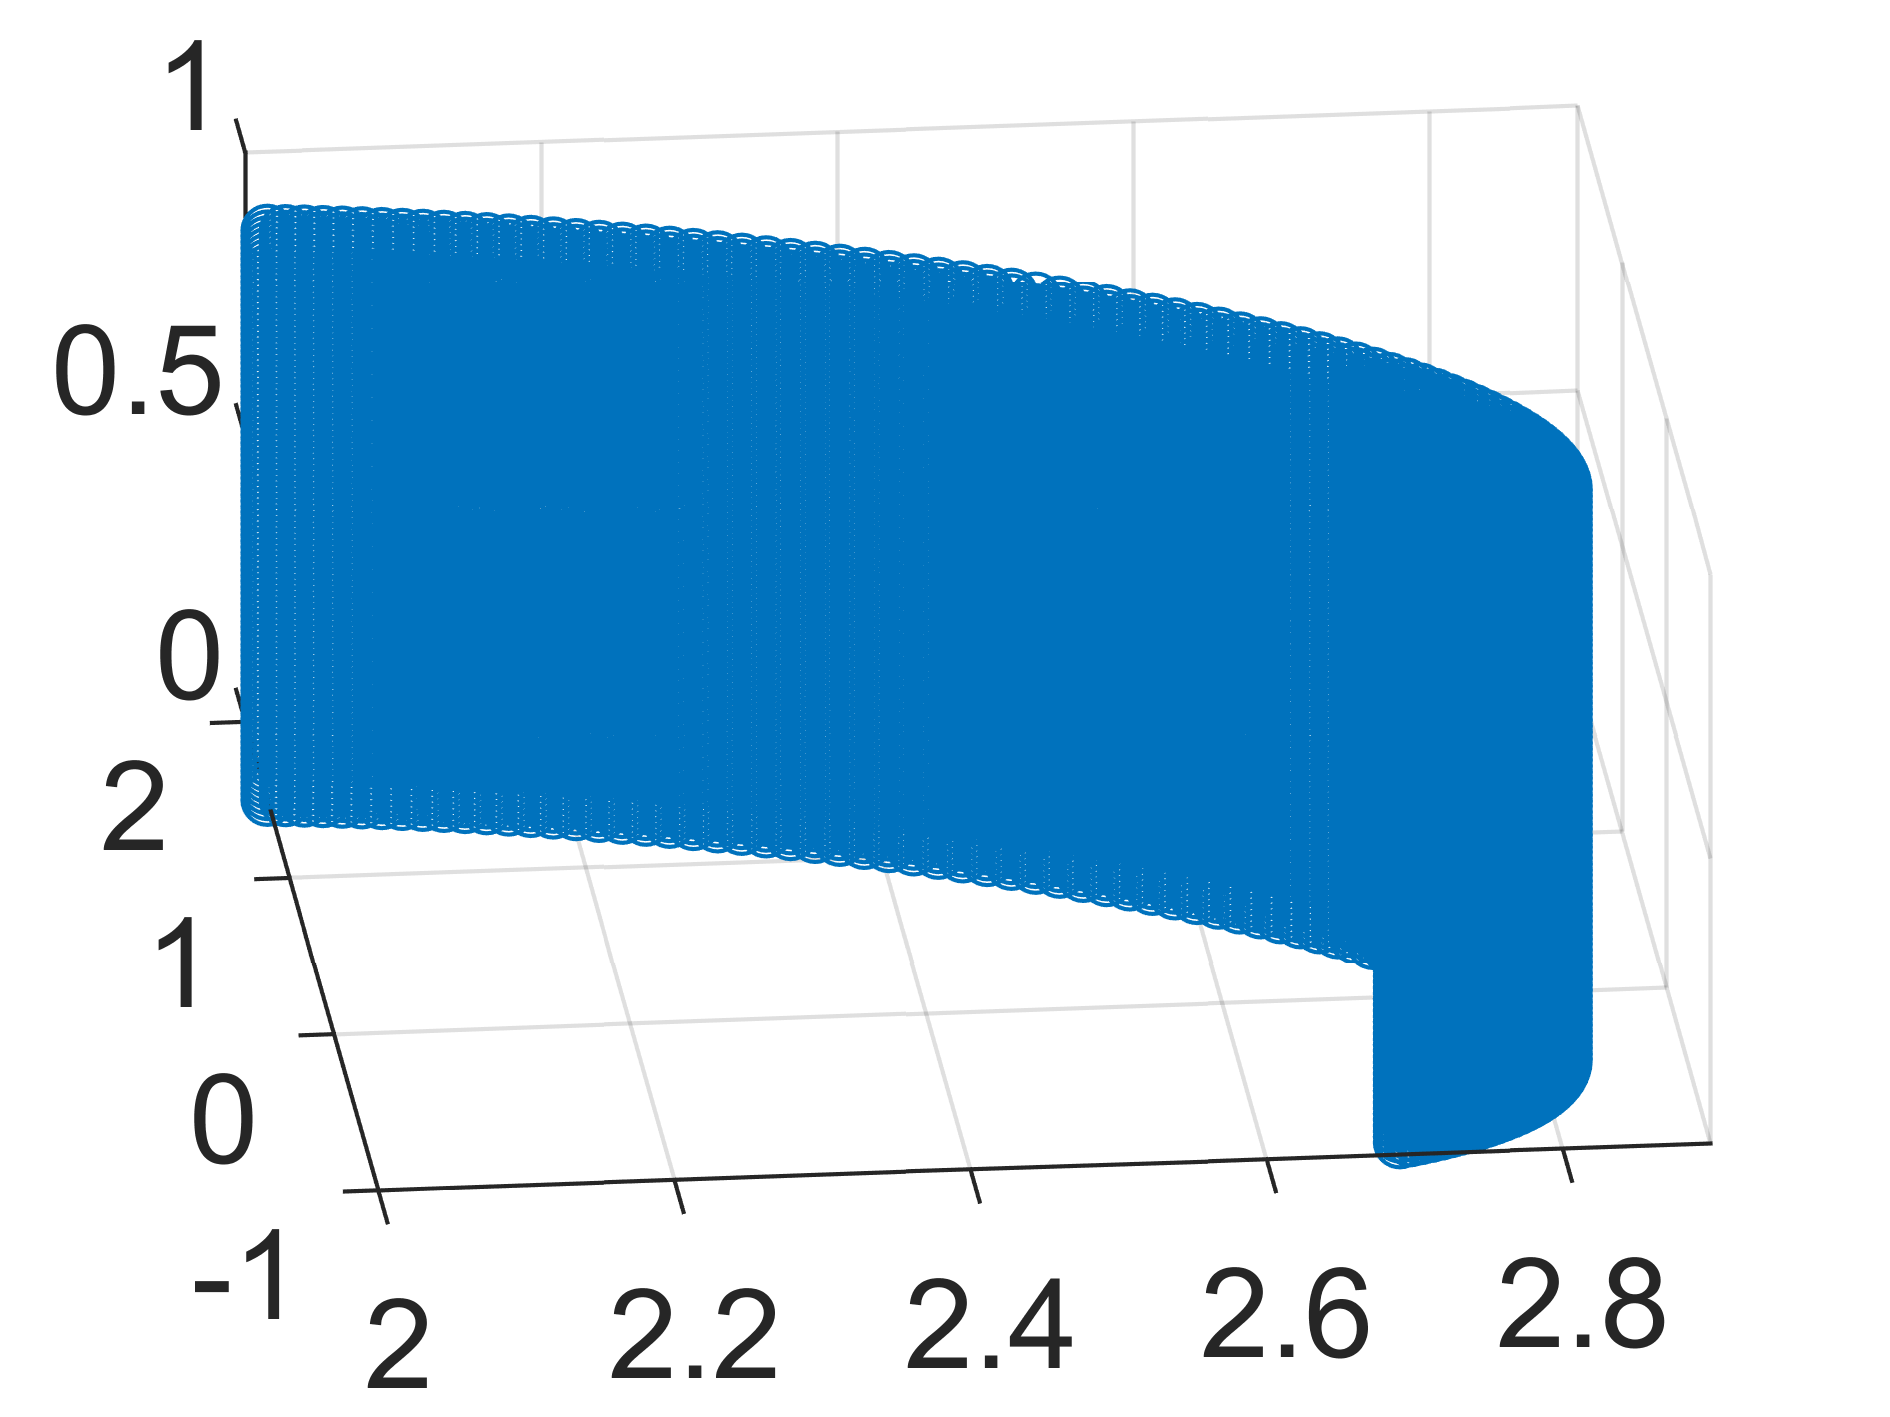
\includegraphics[height=6.5cm,width=1\textwidth,keepaspectratio]{extruding_surface.png}
                % \caption{caption_name}
                \label{fig:extruding_surface.png}
            \end{figure}
        \end{column}
    \end{columns}
\end{frame}

\begin{frame}[t]{Surface made by extruding in Fusion 360}
    \framesubtitle{Video}
    \vspace{-0.6cm}
    \begin{figure}[H]
        \href{run:./videos/extruding_surface_video.mp4}{
            \centering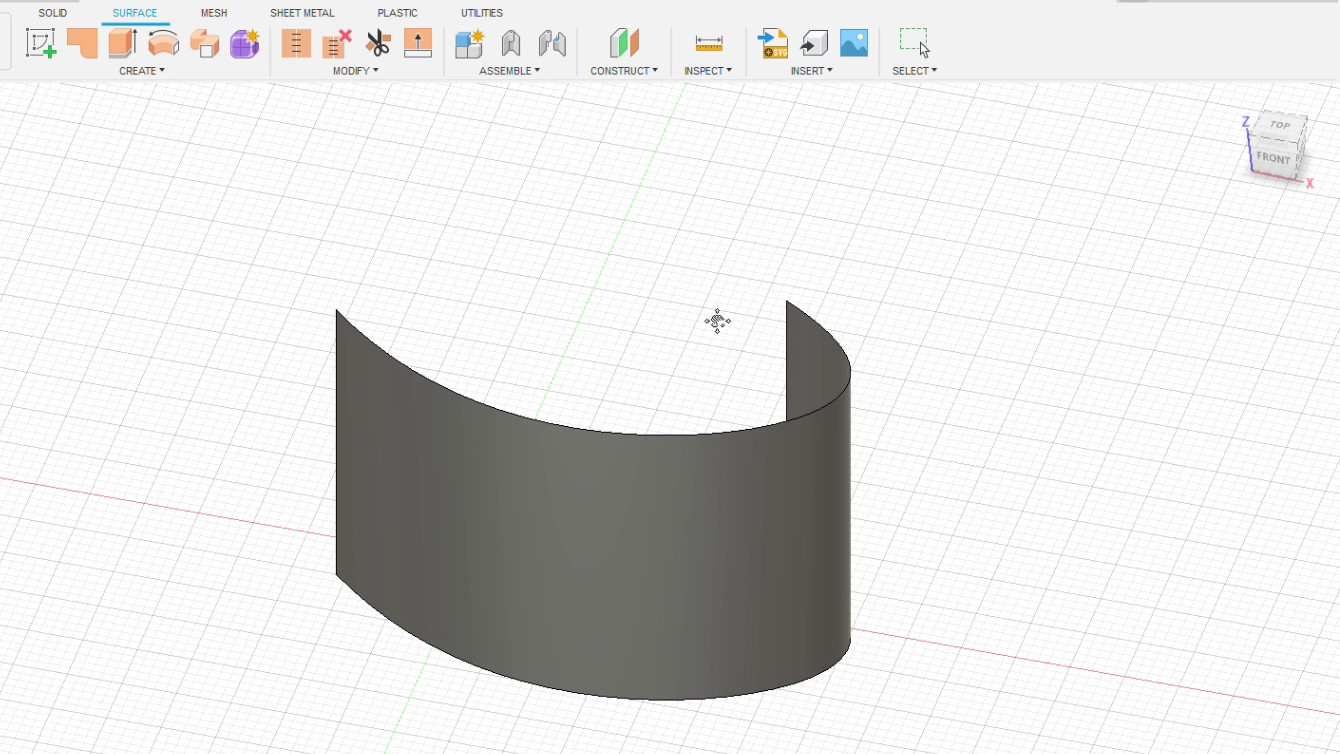
\includegraphics[height=6cm,width=1\textwidth,keepaspectratio]{extruding_surface_video_preview.jpg}}
        % \caption{Click on a picture for a video}
    \end{figure}
\end{frame}

\begin{frame}[t]{Surface made by sweeping}
\framesubtitle{}
    \begin{columns}[T,onlytextwidth]
        \begin{column}{0.49\textwidth}
            \begin{align*}
                \vec{r}(u,v) = \vec{g}(v) + \vec{c}(u) - \vec{g}(v_{min})
            \end{align*}
        \end{column}
        \begin{column}{0.49\textwidth}
            \begin{figure}[H]
                \centering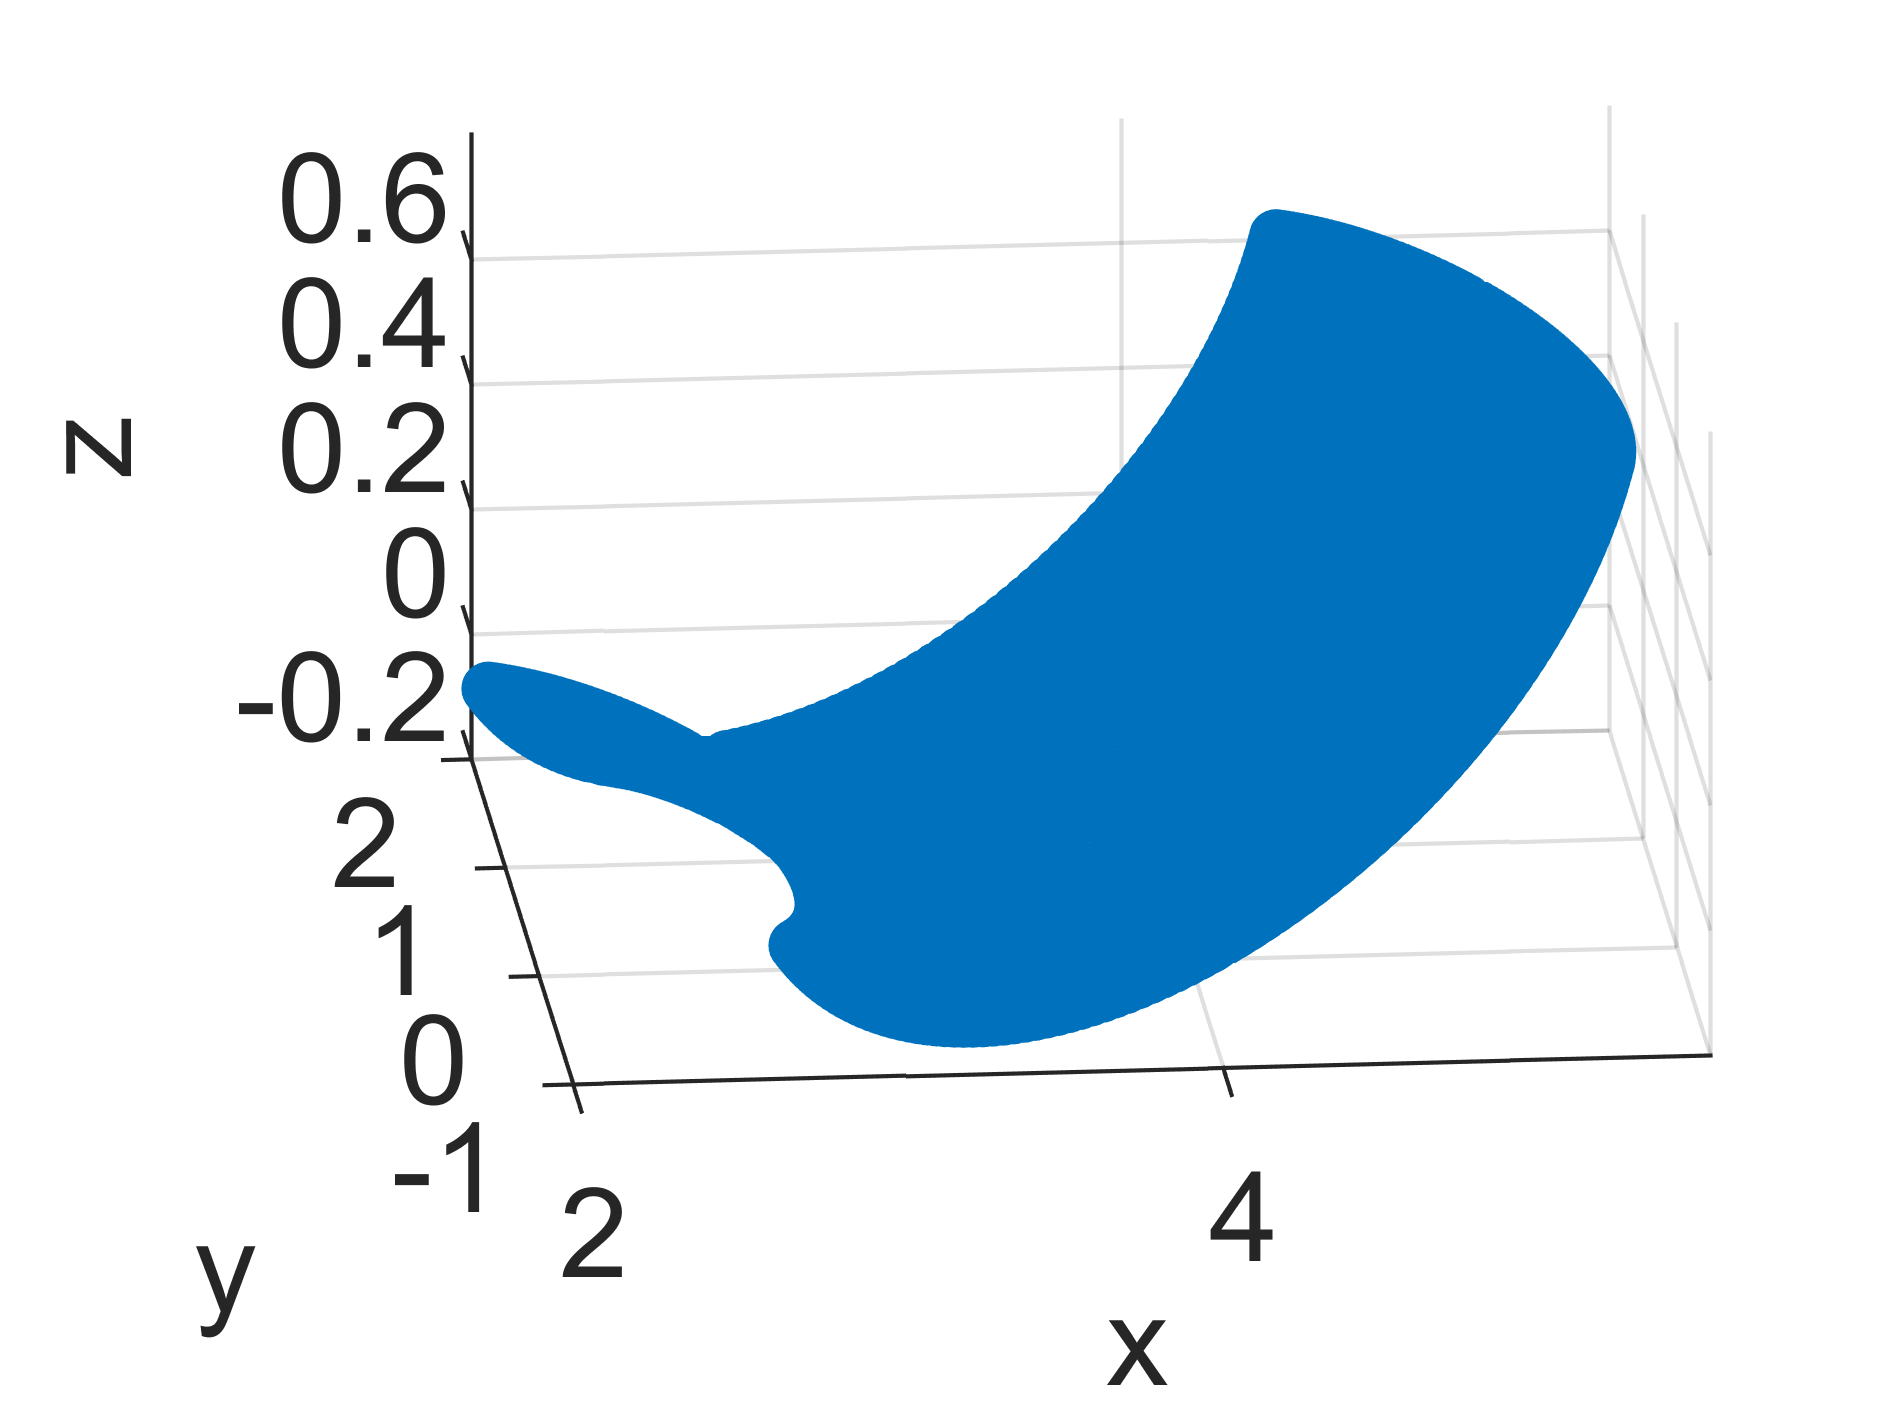
\includegraphics[height=6cm,width=1\textwidth,keepaspectratio]{sweeping_surface.png}
                % \caption{caption_name}
                \label{fig:sweeping_surface.png}
            \end{figure}
        \end{column}
    \end{columns}
\end{frame}

\begin{frame}[t]{Surface made by sweeping in Fusion 360}
    \framesubtitle{Video}
    \vspace{-0.6cm}
    \begin{figure}[H]
        \href{run:./videos/sweep_surface_video.mp4}{
            \centering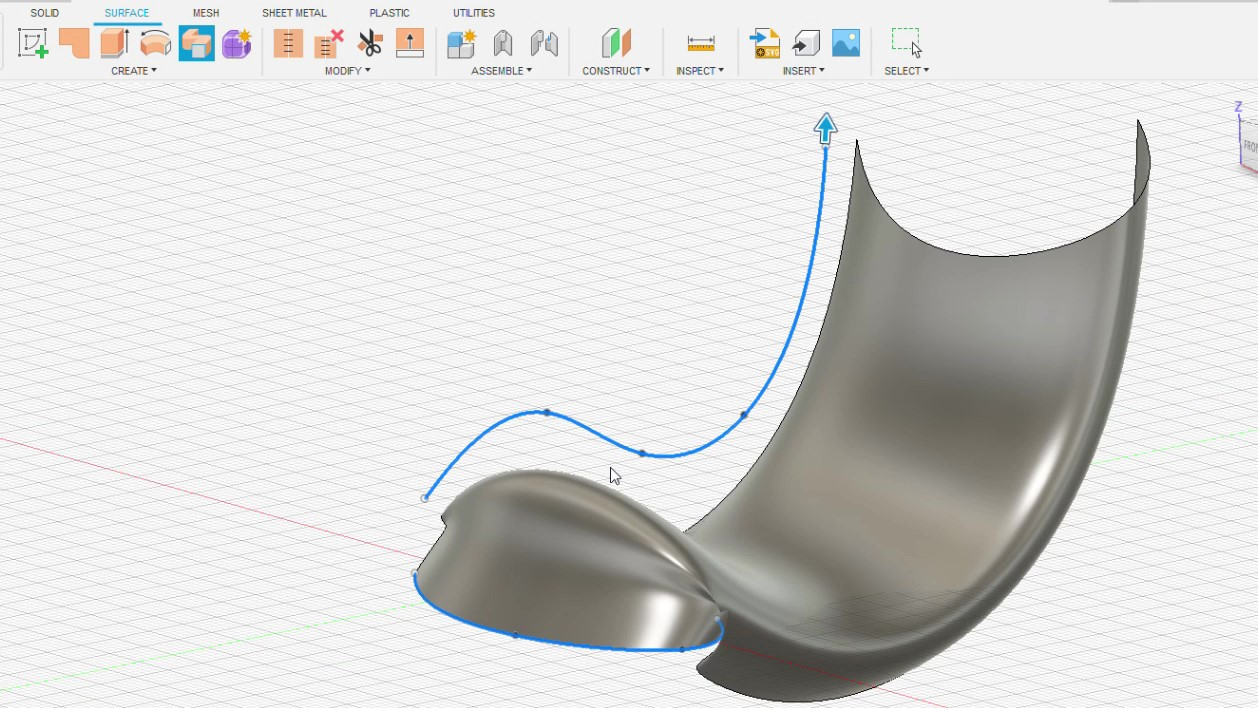
\includegraphics[height=6cm,width=1\textwidth,keepaspectratio]{sweep_surface_video_preview.jpg}}
        % \caption{Click on a picture for a video}
    \end{figure}
\end{frame}

\begin{frame}[t]{Summary}
\framesubtitle{}
\begin{enumerate}
    \item We touched the benefits of a parametric form
    \pause
    \item We know the equation of the line and polyline
    \pause
    \item We heard about spline applications
    \pause
    \item We know 2 types of splines and the difference between them
    \pause
    \item We got acquainted with a proof how correlates conic sections and bezier splines
    \item We know 3 methods of obtaining surfaces
\end{enumerate}

\end{frame}

\begin{frame}[t]{Reference material}
    % \framesubtitle{OnlineMschool}
    \Large
    \begin{itemize}
        \item \href{https://libgen.is/book/index.php?md5=D650EF9E78CBCD3367240A00B610C383}{Geometrical Modeling, Golovanov N.N. (book, rus)}
        \item \href{https://youtu.be/aVwxzDHniEw}{The Beauty of Bézier Curves (video, eng)}
        \item \href{http://wp.doc.ic.ac.uk/bkainz/teaching/60005-co317-computer-graphics/}{Computer Graphics course, lectures notes 12 and 13 (Imperial College London)}
        \item \href{https://www.youtube.com/watch?v=lk3uObcVnN0}{12 Spline Curves (video, eng)}
        \item \href{https://youtu.be/rtwOrZL02M0}{Data Fitting: Polynomial Fitting and Splines, Part 4 (video, eng)}
        \item \href{https://habr.com/ru/post/323442/}{Qubic spline (habr, rus)}
    \end{itemize}
\end{frame}

\fbckg{fibeamer/figs/last_page.png}
\frame[plain]{}

\end{document}